%\motto{Use the template \emph{chapter.tex} to style the various elements of your chapter content.}


\chapter{Quantenhardware}
\label{hardware} % Always give a unique label
% use \chaptermark{}
% to alter or adjust the chapter heading in the running head

\chapterauthor{Dennis Hülsken, Jakob Krumke, Marc Meyer, Daniel Roth, Tom Slatosch}

\abstract{some abstract}

\section{Einführung in Quantenhardwareplattformen}
Die physikalische Realisierung eines Quantencomputers ist maßgeblich durch die Wahl der zugrunde liegenden Hardwareplattform bestimmt. Quantenhardware bildet das technische Fundament für alle quantenlogischen Operationen und beeinflusst entscheidend die Skalierbarkeit, Robustheit und Anwendungsdomänen heutiger und zukünftiger Quantencomputer. Der Begriff „Plattform“ bezeichnet hierbei die physikalischen Systeme, mit denen Qubits realisiert, kontrolliert und gemessen werden. Zwei übergeordnete Klassen haben sich als besonders relevant herausgestellt: Festkörperbasierte und atomare Plattformen \cite{schmaltz2025, homeister2020}.

\subsection{Überblick über Plattformtypen}
\begin{itemize}
\item \textbf{Festkörperplattformen} nutzen mikroskopische Strukturen in festen Materialien – typischerweise Halbleiter oder supraleitende Metalle, um Qubits durch elektrische, magnetische oder optische Eigenschaften zu realisieren. Bekannte Beispiele sind supraleitende Transmon-Qubits, Quantenpunkte und diamantbasierte NV-Zentren.
\item \textbf{Atomare Plattformen} beruhen auf der Manipulation einzelner Atome oder Ionen, die mithilfe elektromagnetischer Felder in Fallen gespeichert und durch Laser- oder Mikrowellenpulse angeregt werden. Dazu zählen Ionenfallen, Neutralatomfallen und photonische Systeme.
\end{itemize}

Diese Plattformen unterscheiden sich signifikant hinsichtlich ihrer technologischen Reife, Kohärenzeigenschaften und praktischen Einsatzmöglichkeiten. Tabelle \ref{tab:plattformvergleich} stellt zentrale Merkmale beider Klassen gegenüber:

\begin{table}[h]
\centering
\caption{Vergleich atomarer und festkörperbasierter Quantenhardwareplattformen}
\label{tab:plattformvergleich}
\begin{tabular}{|p{4cm}|p{5cm}|p{5cm}|}
\hline
\textbf{Aspekt} & \textbf{Atomare Plattformen} & \textbf{Festkörperplattformen} \\
\hline
Beispiele & Ionenfallen, Rydberg-Atome & Transmon-Qubits, NV-Zentren, Quantenpunkte \\
Qubit-Implementierung & Einzelatome oder Ionen in Fallen & Elektronen-/Spinzustände in Materialien \\
Kohärenzzeiten & Sehr lang (bis zu Minuten) & Kürzer (µs–ms) \\
Steuerung & Laser- und Mikrowellenfelder & Elektrische/optische Signale, Mikrowellen \\
Herstellung & Komplexe atomare Präparation & Standardisierte Halbleiterfertigung \\
Skalierbarkeit & Eingeschränkt durch optische Systeme & Gute Integrationsmöglichkeiten \\
Anwendungen & Metrologie, Quantensimulation & Algorithmische Anwendungen, Optimierung \\
\hline
\end{tabular}
\end{table}


\subsection{Technologischer Reifegrad und Herausforderungen}
Laut der „Schwerpunktstudie Quantenökosysteme“ des Fraunhofer ISI befinden sich supraleitende Systeme (v.a. Transmon-Qubits) sowie Ionenfallen derzeit auf dem höchsten technologischen Entwicklungsstand. Beide Plattformen konnten bereits fehlerkorrigierte Gatter demonstrieren, wenngleich unter hohem technologischem Aufwand \cite{schmaltz2025}.

Andere Ansätze wie photonische Qubits oder NV-Zentren bieten teils attraktive Eigenschaften (z.B. Raumtemperaturbetrieb oder geringe Dekohärenzanfälligkeit), sind jedoch noch mit praktischen Limitierungen bei Skalierung, Adressierbarkeit oder Gatterqualität konfrontiert \cite{homeister2020}.

Die derzeit gängigen Quantencomputer zählen zur Klasse der sogenannten \textit{Noisy Intermediate-Scale Quantum}-Systeme (NISQ). Diese verfügen über 50–150 Qubits, erlauben jedoch keine vollumfängliche Fehlerkorrektur. Anwendungen beschränken sich auf experimentelle Algorithmen mit begrenzter Komplexität \cite{schmaltz2025, homeister2020}.

Ein Durchbruch in Richtung großskaliger, universeller Quantencomputer wird eine massive Erhöhung der Qubit-Zahl, Schätzungen gehen von $10^5$ bis $10^6$ Qubits aus, sowie Fortschritte bei Fehlertoleranz und Architektur erfordern \cite{schmaltz2025}.

\subsection{Ausblick auf die Kapitelstruktur}
Die folgende Gliederung dieser Arbeit orientiert sich an den bedeutendsten physikalischen Plattformen des aktuellen Forschungsstandes. Jede Plattform wird hinsichtlich ihrer physikalischen Grundlagen, technischer Implementierung, Herausforderungen und Perspektiven systematisch analysiert. Die Kapitel im Überblick:

\begin{itemize}
\item \textbf{Kapitel 1.2: Supraleitende Qubits}
\item \textbf{Kapitel 1.3: Ionenfallen-Qubits}
\item \textbf{Kapitel 1.4: Diamantbasierte Qubits (NV-Zentren)}
\item \textbf{Kapitel 1.5: Weitere Plattformen} 
\item \textbf{Kapitel 1.6: Praxisbeispiel IBM Q}
\end{itemize}

Dieses Einführungskapitel legt somit den Grundstein für ein vertieftes Verständnis der komplexen und heterogenen Hardwarelandschaft im Quantencomputing. Es zeigt, dass die Wahl der Plattform nicht nur technische, sondern auch strategische Bedeutung für den weiteren Fortschritt in Forschung und Anwendung besitzt.

\section{Supraleitende Qubits}
Supraleitende Quantencomputer nutzen die Prinzipien der Quantenmechanik und die einzigartigen Eigenschaften von Supraleitern, um Quantenberechnungen durchzuführen. Diese Systeme sind darauf ausgelegt, komplexe Aufgaben in Bereichen wie Quantenchemie, Simulation, Kryptographie und Optimierung zu bewältigen, was ihnen potenzielle Vorteile gegenüber klassischen Systemen verschafft. Die Realisierung dieser Rechenvorteile hängt jedoch von der effizienten und skalierbaren Ausführung von Quantenprogrammen auf robuster Hardware ab, die für Quantenoperationen konzipiert ist.
\subsection{physikalisches Prinzip supraleitende qubits}
\subsection{Implementierung von Quantenlogik}
\subsubsection{Grundlegende Prinzipien und Typen}
Die fundamentalen Einheiten der Quanteninformation in supraleitenden Systemen sind supraleitende Qubits, die als künstliche Atome mit quantisierten Energieniveaus fungieren. Diese Qubits werden typischerweise aus supraleitenden Schaltkreisen gefertigt, die Materialien wie Aluminium oder Niob verwenden und bei extrem niedrigen Temperaturen, nahe dem absoluten Nullpunkt (ca. 15 Millikelvin), betrieben werden(The ultimate Guide to Superconducting Quantum Computers, 2025). Die Supraleitung, die bei diesen Temperaturen erreicht wird, gewährleistet einen widerstandslosen Stromfluss, was für die Aufrechterhaltung der Kohärenz der Qubits und ihrer Quantenzustände unerlässlich ist.
\\\\
Ein supraleitendes Qubit besteht häufig aus einem Induktor und einem Kondensator (LC-Oszillator), die durch einen Josephson-Kontakt verbunden sind. Der Josephson-Kontakt ist ein entscheidendes nichtlineares Element, das eine Anharmonizität in das Energiespektrum des Schaltkreises einführt. Diese Anharmonizität ist von größter Bedeutung, da sie sicherstellt, dass nur die beiden niedrigsten Energiezustände - der Grundzustand 0 and der erste angeregte Zustand 1 - als Qubit-Zustände dienen. Ohne diese Nichtlinearität würde der Quanten-LC-Schaltkreis als einfacher harmonischer Oszillator mit äquidistanten Energieniveaus fungieren, wodurch eine isolierte Zwei-Niveau-System-Nutzung als Qubit unmöglich wäre. Die präzise technische Gestaltung des Josephson-Kontakts und die Auswahl des supraleitenden Materials sind daher nicht nur Fertigungsdetails, sondern grundlegend für die Schaffung eines stabilen und adressierbaren Zwei-Niveau-Systems. Sie bestimmen die grundlegenden Eigenschaften des Qubits wie Anharmonizität, Kohärenzzeit und Rauschresistenz, die für zuverlässige Quantenoperationen unerlässlich sind. Die Betriebsumgebung von supraleitenden Quantencomputern erfordert extrem niedrige Temperaturen, typischerweise im Bereich von 10 bis 20 Millikelvin(mK). Um diese Temperaturen zu erreichen, werden komplexe Kühlsysteme, meist Dilution Refridgerators, benötigt. Um eine solch extreme Kühlung zu ermöglichen, wird die Phasenmischung von Helium-3 und Helium-4 verwendet. Eine genauere Beschreibung zum Aufbau der Kühlsysteme und deren Funktionsweise sowie aktuelle Modelle, sind im Kapitel 1.2.4 zu finden.
\\\\
Der am häufigsten verwendete Qubit-Typ, bei supraleitenden Quantencomputern, ist das Transmon-Qubit. Dieser Transmon-Qubit weißt einen spezifische Hardwareaufbau auf. Er ist eine Weiterentwicklung des Cooper-Pair-Box-Qubits und besteht im Wesentlichen aus einem Josephson-Kontakt, der parallel zu einem relativ großen Shunt-Kondensator geschaltet ist. Dieser Kondensator, oft in einer \glqq Kreuz\grqq{}-Form (bekannt als Xmon), ist entscheidend, da er die Empfindlichkeit des Qubits gegenüber Ladungsrauschen drastisch reduziert und somit längere Kohärenzzeiten ermöglicht. Die typischen Betriebsfrequenzen von Transmonen liegen um 5 GHz, können aber in-situ zwischen etwa 4 und 6 GHz abgestimmt werden. Für die Frequenzabstimmung werden häufig zwei Josephson-Kontakte parallel in einer SQUID-Schleife (Superconducting QUantum Interference Device) angeordnet. Das Anlegen eines externen Magnetflusses an diese Schleife ermöglicht die dynamische Anpassung der effektiven Josephson-Energie und damit der Resonanzfrequenz des Qubits. (Roth Thomas, 04.2023). Ein alternativer Qubit-Typ ist das Fluxonium-Qubit. Dieses Qubit gewinnt aktuell an Interesse, da es durch einen leicht abgeänderten Aufbau höhere Kohärenzzeiten und hohe Gatter-Fidelitäten erreichen kann. Der Herstellungsprozess dieser Qubits umfasst mehrere Schritte, darunter lithographische Strukturierung, Metallabscheidung, Nass- oder Trockenätzen und die kontrollierte Oxidation von Supraleiterfilmen zur Bildung der Josephson-Kontakte. Fortschritte in der industriellen Halbleiterfertigung, wie optische Lithographie und reaktives Ionenätzen auf großen 300-mm-Siliziumwafern, zeigen vielversprechende Wege zur Skalierung mit hohen Ausbeuten an funktionsfähigen Qubits auf. (Kady Bentley, 2025)

\begin{figure}[ht]
    \centering
    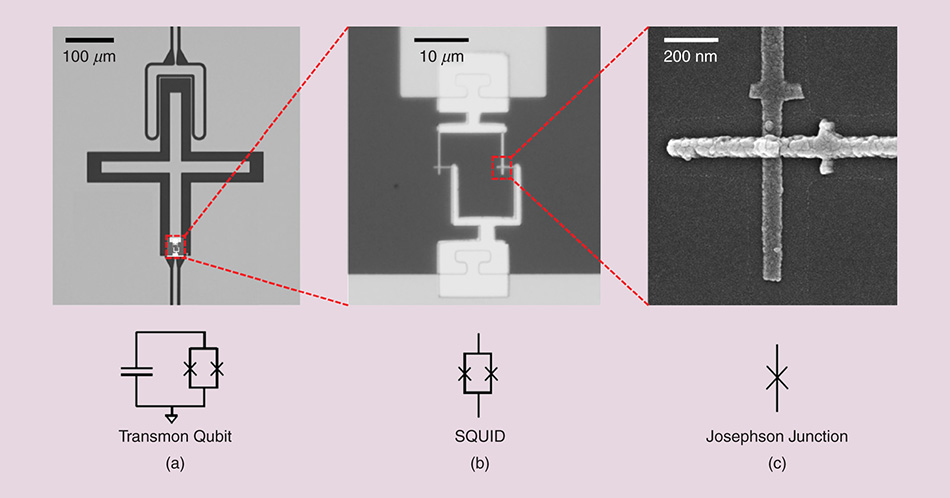
\includegraphics[width=1\textwidth]{images/quanten-hardware/Transmon Qubit.jpg}
    \caption{(a) vollständiges Qubit, (b) Zoom auf die SQUID-Schleife, (c) Josephson-Kontakt}
    \label{fig:transom_image}
    \end{figure}

\subsubsection{Ein-Qubit-Gatter}
Ein-Qubit-Gatter sind die grundlegendsten Operationen in einem Quantencomputer und ermöglichen die gezielte Manipulation des Zustands eines einzelnen Qubits.Diese Gatter, die Rotationen auf der Bloch-Kugel darstellen (z.B. X-, Y- und Z-Rotationen), werden in supraleitenden Quantencomputern durch die präzise Anwendung von Mikrowellenpulsen realisiert.
\\\\
Ein-Qubit-Gatter werden durch das Anlegen von Mikrowellenpulsen realisiert, die auf die Übergangsfrequenz des Qubits abgestimmt sind. Diese Pulse induzieren kohärente Oszillationen, sogenannte Rabi-Oszillationen, zwischen den \big \vert0⟩ und \big \vert1⟩ Zuständen des Qubits. Die Dauer und Phase dieser Pulse bestimmen die Art der Rotation auf der Bloch-Kugel. Beispielsweise können X- und Y-Rotationen durch entsprechend phasenverschobene Mikrowellenpulse erzeugt werden. Z-Rotationen können oft virtuell durch Software implementiert werden, indem die Phase der nachfolgenden Mikrowellenanregungen angepasst wird, was keine physische Pulsdauer erfordert (Characterizing Superconductiong Qubits).\\\\Der Signalpfad für die Qubit-Steuerung ist eine komplexe Kette, die von Raumtemperatur-Elektronik bis zum Qubit im Dilutionskühler reicht. Die Erzeugung der präzisen Mikrowellenpulse beginnt bei Raumtemperatur mit Arbitrary Waveform Generators (AWGs) und Digital-Analog-Wandlern (DACs), die die Basisband-Pulswellenformen erzeugen. Diese Basisband-Signale werden dann mittels Mischer mit einem lokalen Oszillator (LO) zu Mikrowellenfrequenzen (typischerweise 2-10 GHz) hochkonvertiert (Bao Zenghui, 2024). Die Mikrowellensignale werden über Koaxialkabel durch die verschiedenen Temperaturstufen des Kryostaten (z.B. 3K, 1K, 100mK, 10mK) zum Qubit geleitet. Entlang dieses Pfades sind Dämpfungsglieder und Filter angebracht, die an den jeweiligen Temperaturstufen thermisch verankert sind. Ihre Funktion ist es, das von Raumtemperatur eindringende Rauschen zu reduzieren und unerwünschte Frequenzen zu unterdrücken, die die Qubit-Kohärenz stören könnten. Am kältesten Punkt (mK-Stufe) erreichen die Signale den Qubit-Chip über On-Chip-Drive-Lines, die kapazitiv oder induktiv mit den Qubits gekoppelt sind. Die Skalierung dieser Verkabelung stellt eine erhebliche Herausforderung dar, da jede zusätzliche Leitung Wärme in den Kryostaten einbringt und die Kühlleistung begrenzt ist. Dies treibt die Forschung an monolithisch integrierter Steuerungselektronik direkt auf dem Qubit-Chip voran, um den Verkabelungsaufwand und die Wärmelast zu reduzieren (Bao Zenghui, 2024).

\subsubsection{Zwei-Qubit-Gatter}
Zwei-Qubit-Gatter sind für die Durchführung komplexer Quantenalgorithmen unerlässlich, da sie die Verschränkung von Qubits ermöglichen. Ihre Implementierung erfordert eine kontrollierte Wechselwirkung zwischen den Qubits, die auf verschiedene Weisen hardwareseitig realisiert werden kann. Die Entwicklung der Zwei-Qubit-Kopplung hat sich von direkten zu vermittelten, dynamisch steuerbaren Interaktionen entwickelt, um Skalierungs- und Fehlerreduktionsanforderungen zu erfüllen.\\\\
\textbf{Kapazitive Kopplung:}\\
Die kapazitive Kopplung ist eine grundlegende Methode zur Realisierung von Zwei-Qubit-Gattern. Sie wird physisch durch die Platzierung von leitenden Strukturen (Pads oder \grqq{}Coupler Arms\grqq{} ) in unmittelbarer Nähe der Qubits auf dem Chip erreicht, wodurch eine elektrische Kopplung entsteht. Häufig werden hierfür interdigitierte Kondensatoren oder direkte Pads verwendet, die eine effektive Kapazität zwischen den Qubits herstellen.\\
Eine Herausforderung bei der direkten kapazitiven Kopplung in größeren Systemen ist das unerwünschte Übersprechen (Crosstalk) zwischen nicht benachbarten Qubits, das die Gatter-Fidelität beeinträchtigen kann. Um dies zu mindern, wurden fortgeschrittene Designs entwickelt, die \grqq{}Waveguide Extenders\grqq{} oder \grqq{}Coupler Arms\grqq{} mit interdigitierten oder Gap-Kondensatoren nutzen, um die Kopplung über größere physische Distanzen zu vermitteln und gleichzeitig das Übersprechen zu reduzieren. Diese Extender ermöglichen eine flexiblere Platzierung der Qubits auf dem Chip und schaffen Raum für zusätzliche Komponenten wie Ausleseresonatoren und Purcell-Filter.
\\\\
\textbf{Resonatorbasierte Kopplung (Quantenbus):}\\
Eine weit verbreitete und skalierbare Technik zur Kopplung mehrerer Qubits ist die Verwendung eines Mikrowellenresonators als \grqq Quantenbus\grqq{}. Dieser Resonator fungiert als Vermittler und ermöglicht es Qubits, miteinander zu interagieren, selbst wenn sie nicht direkt benachbart sind. Die Interaktion erfolgt über den Austausch virtueller Photonen mit dem Resonator. Dieses Konzept wird als \grqq Circuit QED\grqq{} (Quantenelektrodynamik in Schaltkreisen) bezeichnet, analog zur optischen Kavität-QED.\\
Durch gezieltes Abstimmen der Qubits in und aus der Resonanz mit dem Bus können verschränkende Zwei-Qubit-Gatter wie Controlled-NOT (CNOT) oder iSWAP implementiert werden. Der Quantenbus bietet eine effektive All-to-All-Konnektivität zwischen einer Gruppe von Qubits, was für bestimmte Algorithmen vorteilhaft ist. Die \grqq Quantum Bus\grqq{}-Architektur ist nicht nur ein Kopplungsmechanismus, sondern eine grundlegende architektonische Wahl, die flexible und höhergradige Konnektivität zwischen Qubits ermöglicht. Diese Modularität ist entscheidend für die Entwicklung von Quantenprozessoren, die an spezifische Algorithmen und Fehlerkorrekturcodes angepasst werden können, wodurch die Einschränkungen von festen Topologien und spärlicher Konnektivität in größeren Quantensystemen direkt angegangen werden.

\subsection{Beispiele supraleitende Qubits}
Die Entwicklung supraleitender Quantenprozessoren hat in den letzten Jahren beeindruckende Fortschritte gemacht, was sich in der steigenden Anzahl von Qubits und der Demonstration komplexer Quantenoperationen zeigt. Zwei herausragende Beispiele sind Googles Sycamore und IBMs Eagle Prozessoren.
\\\\
\textbf{Google Scaymore}\\\\
Der Google Sycamore Prozessor, der 2019 vorgestellt wurde, war ein 53-Qubit-System, das auf supraleitenden Transmon-Qubits basierte. Obwohl der Chip physisch 54 Qubits umfasste, war einer während der entscheidenden Tests inaktiv, wodurch 53 Qubits für die Demonstration zur Verfügung standen. Die Qubits sind in einem rechteckigen Gitter angeordnet und weisen eine Nearest-Neighbor-Kopplung auf. Google verwendete eine spezielle Variante des Transmon-Qubits, den sogenannten Xmon, der sich durch eine kreuzförmige Kapazität auszeichnet, die eine verbesserte Konnektivität ermöglicht.\\\\
Die Konnektivität zwischen den Qubits im Sycamore-Prozessor wurde durch eine \grqq Tunable Coupling Architecture\grqq{} realisiert. Diese Architektur nutzte abstimmbare Koppler-Transmonen, die es ermöglichten, die Verbindungen zwischen den Qubits bei Bedarf dynamisch \grqq ein- und auszuschalten\grqq{}. Im Sycamore-Prozessor waren 88 solcher Transmon-Koppler vorhanden, die die Konnektivität zwischen den Qubit-Paaren herstellten. Ein weiteres wichtiges Designmerkmal des Sycamore-Chips war sein \grqq Flip-Chip\grqq{}-Design. Hierbei ist das Qubit-Array auf einem separaten Steuerchip gestapelt, der alle Steuer- und Ausleseleitungen enthält. Dieses 3D-Integrationskonzept verbesserte die Skalierbarkeit im Vergleich zu herkömmlichen 2D-Designs erheblich, da es die Verdrahtungsdichte auf der Qubit-Ebene reduzierte.\\\\
Die Hardware des Sycamore-Prozessors wurde speziell für hohe Fidelität bei Ein- und Zwei-Qubit-Operationen entwickelt. Google berichtete von der Durchführung von 1.113 Ein-Qubit-Gattern und 430 Zwei-Qubit-Gattern in den größten Schaltkreisen, mit einer erwarteten Gesamtfidelität von etwa 0,2\%. Obwohl dieser Wert scheinbar niedrig war, reichte er aus, um eine messbare Korrelation mit der korrekten Quantenwahrscheinlichkeitsverteilung zu zeigen. Die Demonstration der \grqq Quantum Supremacy\grqq{} für eine spezifische, rechenintensive Stichprobenaufgabe (Sampling the output of a random quantum circuit) in 200 Sekunden, für die klassische Supercomputer schätzungsweise 10.000 Jahre benötigt hätten, war ein wissenschaftlicher Meilenstein. Dieses Ergebnis erforderte eine minutiöse Minimierung von Fehlern durch synchronisierte und kalibrierte Qubit-Operationen, um die Quantenkohärenz über die Dauer der Berechnung aufrechtzuerhalten.
\\\\
\textbf{IBM Eagle}\\\\
Der IBM Eagle Prozessor, der Ende 2021 vorgestellt wurde, war der erste Quantenchip, der die 100-Qubit-Marke überschritt, mit insgesamt 127 Qubits. Auch dieser Prozessor basiert auf supraleitenden Transmon-Qubits. Das Layout des Eagle-Chips zeichnet sich durch eine \grqq Heavy-Hex\grqq{}-Topologie aus. In diesem Layout ist jedes Qubit mit maximal zwei oder drei Nachbarn verbunden, was eine tessellierende hexagonale Struktur bildet, im Gegensatz zum quadratischen Gitter von Google Sycamore. Die Wahl dieser Topologie zielt darauf ab, unerwünschte Wechselwirkungen und Übersprechen zwischen benachbarten Qubits zu reduzieren, indem sie nicht zu dicht beieinander gepackt werden.\\\\
Eine der wichtigsten technischen Innovationen im Eagle-Design ist die Multi-Layer-Verdrahtung (MLW) innerhalb des Interposers. Während frühere IBM-Chips eine zweischichtige Architektur mit einem Qubit-Chip nutzten, der auf einen Interposer bump-gebondet war, integriert Eagle zusätzliche Verdrahtungsebenen im Interposer selbst. Dies ermöglicht es, Steuer- und Auslesesignale tief in den Chip zu leiten, ohne die 2D-Oberfläche zu überfüllen. Die MLW-Ebene besteht aus mehreren Metallschichten mit dazwischenliegenden, planaren Dielektrika und kurzen Verbindungen, sogenannten Vias, die die Metallebenen verbinden.\\\\ 
Zusätzlich integriert der Eagle-Prozessor Durchkontaktierungen (Through-Silicon Vias, TSVs) sowohl in den Qubit- als auch in den Interposer-Chips. Im Qubit-Chip unterdrücken TSVs unerwünschte Resonanzmoden (\grqq Box Modes\grqq{}) und bilden \grqq Via-Zäune\grqq{} zwischen Qubits und anderen empfindlichen Mikrowellenstrukturen, die als Faraday-Käfige wirken und kapazitives Übersprechen verhindern. Im Interposer-Chip ermöglichen TSVs die Signalübertragung zwischen den MLW-Ebenen und den gewünschten Stellen im Chip. Diese MLW- und TSV-Technologien bieten eine natürliche Abschirmung gegen Übersprechen, was zu einer Reduzierung des Übersprechens im Vergleich zu früheren Architekturen wie Falcon führt.\\\\
Eine weitere entscheidende Skalierungsinnovation im Eagle ist das Auslese-Multiplexing. Frühere supraleitende Prozessoren benötigten für jedes Qubit eine dedizierte Mikrowellen-Steuerleitung und einen separaten Ausleseresonator, was bei mehr als einigen Dutzend Qubits unpraktisch wurde. Eagle hingegen nutzt Frequenz-Multiplexing, sodass mehrere Qubits dieselbe Ausleseleitung auf unterschiedlichen Frequenzen teilen können. Dies reduziert die Anzahl der Koaxialkabel und Steuerhardware-Kanäle im Kryostaten drastisch und erleichtert die physische Verkabelung von 127 Qubits erheblich. Die Kombination aus Heavy-Hex-Topologie, mehrschichtiger 3D-Verdrahtung und multiplexiertem Auslesen zeigt, wie IBM die Herausforderung der Quantenskalierung aus mehreren Blickwinkeln angeht – Qubit-Layout, Steuerinfrastruktur und Fertigung mussten sich weiterentwickeln, um einen 127-Qubit-Prozessor zu ermöglichen.


\subsection{Herausforderungen supraleitende Qubits}
Die technische Realisierung supraleitender Quantencomputer ist mit einer Reihe komplexer Herausforderungen verbunden, die insbesondere im Bereich der kryogenen Kühlung, der Skalierung von Qubit-Systemen und der physikalischen Signalverarbeitung auftreten und maßgeblich über die Umsetzbarkeit großskaliger Quantenprozessoren entscheiden.
\\\\
Der Betrieb supraleitender Qubits erfordert extrem niedrige Temperaturen, typischerweise unter 15 Millikelvin (mK), um die Kohärenz aufrechtzuerhalten und die Supraleitung zu ermöglichen.(The ultimate Guide to Superconducting Quantum Computers, 2025). Diese Bedingungen werden durch spezialisierte Kühlsysteme, hauptsächlich Verdünnungskryostate, erreicht. Innerhalb eines Verdünnungskryostat befinden sich die Qubits auf der kältesten Stufe (~10 mK), während die Mikrowellenelektronik auf höheren Temperaturstufen (1 K, 4 K) angeordnet ist. (What Is Cryogenic Quantum Computing and Why It Matters, 2025). Umfassende Abschirmung und Filterung sind entscheidend, um elektromagnetische Interferenzen zu verhindern und thermisches Rauschen zu unterdrücken, das die fragilen Quantenzustände stören und Dekohärenz verursachen kann. Die kryogene Umgebung ist somit nicht nur ein passives Kühlsystem, sondern eine aktive und komplexe Infrastruktur, die die empfindlichen Quantenzustände grundlegend ermöglicht und schützt. Ihre Rolle geht über die reine Kühlung hinaus, da sie aktiv die notwendige Quantenkohärenz aufrechterhält, indem sie verschiedene Formen von Umgebungsrauschen (thermisch, elektromagnetisch) mindert. Verdünnungskryostate sind spezialisierte kryogene Geräte, die die einzigartigen Eigenschaften eines Gemischs aus den Helium-Isotopen Helium-3 und Helium-4 nutzen, um kontinuierlich Temperaturen von bis zu 2 mK zu erreichen. Historisch gesehen wurden \grqq nasse\grqq{} Verdünnungskryostate verwendet, die eine kontinuierliche Versorgung mit flüssigem Helium zur Vorkühlung benötigten. Diese Systeme waren effektiv, aber mit hohen Betriebskosten und logistischem Aufwand verbunden. Seit etwa 2010 hat sich ein signifikanter Wandel hin zu kryogenfreien (\grqq trockenen\grqq{}) Systemen vollzogen. Diese trockenen Systeme verwenden geschlossene Pulskühlröhren (Pulse Tube Refrigerators, PTRs) zur Vorkühlung auf etwa 4 K, wodurch die Notwendigkeit einer externen Flüssigheliumversorgung entfällt. Der Übergang zu kryokogenfreien Verdünnungskryostaten ist nicht nur im Trend sondern auch strategisch notwendig für die Skalierung von Quantencomputern. Trockene Systeme bieten kontinuierlichen Betrieb und eliminieren die Notwendigkeit des Nachfüllens von Flüssighelium, was längere und unterbrechungsfreie Quantenexperimente ermöglicht und die Betriebseffizienz erhöht. Allerdings geht dieser Vorteil oft mit erhöhten mechanischen Vibrationen von den Pulskühlern einher. Trotz dieser Vibrationsherausforderung ist der Wechsel zu trockenen Systemen für die Skalierbarkeit unerlässlich, da er längere, unterbrechungsfreie Experimente ermöglicht und die Betriebseffizienz für größere Quantensysteme verbessert. Die Hersteller investieren daher stark in Vibrationsdämpfungstechniken, um diesen Nachteil zu mindern(J.Rothe, 2025).
\\\\
Aktuelle Branchenführer verwenden unterschiedliche Kühlsysteme von verschiedenen Anbietern um die individuellen Anforderungen zu erfüllen. IBM hat sich für das im Dezember 2023 erste modulare Quantencomputer System für das Kühlsystem \glqq KIDE Cryogenic Platform\grqq{} von dem finnischen Unternehmen Bluefors entschieden. Dieses System ist ein kryogenfreies System, dass auf die Verbindung mehrere Prozessoren ausgelegt ist. Hier wird der von IBM gesetzte Fokus auf skalierbare und modulare Systeme deutlich. Um die riesige Anzahl an Qubits kühlen zu können werden hier neun Pulskühlröhren verwendet, die dafür sorgen verschiedene Temperaturstufen versorgen zu können (Bluefors, 2023). Durch die Nutzung von Pulskühlröhren anstelle von flüssigem Helium können dabei Kühlzeiten von bis zu 3 Jahren realisiert werden. Um modular zu bleiben, wurde KIDE als hexagonale Kammer mit Zugangstüren für Wartung und Möglichkeiten mehrere Cryostat-Einheiten zu koppeln konzipiert. (IBM Quantum, 2024). Ergänzend arbeitet IBM aktuell an dem Goldeye-Projekt mit dem Ziel einen \glqq Super-Kühlschrank\grqq{} mit 1,7 Kubikmetern Volumen zu entwickeln um zukünftig größere Quantensysteme kühlen zu können. (Pat Gumann, Jerry Chow, 2022)\\\\
Google und Intel setzen ebenfalls auf kryogene Plattformen von Bluefors um ihre supraleitenden zu betreiben \cite{noauthor_cryogenic_2025}.
\\\\
\textbf{Skalierbarkeit}\\\\
Ohne extreme Kühlung können supraleitende Qubits nicht funktionieren. Folglich ist jedes Streben nach Skalierung auf dieser Plattform untrennbar mit der Fähigkeit verbunden, diese strengen kryogenen Bedingungen über eine exponentiell wachsende Anzahl von Qubits und deren zugehöriger Steuerinfrastruktur aufrechtzuerhalten und zu verwalten. Diese grundlegende Einschränkung bestimmt viele nachfolgende Hardware-Designentscheidungen und stellt eine primäre Herausforderung dar, die angegangen werden muss, bevor andere Skalierungsprobleme effektiv gelöst werden können.\\\\
Unternehmen wie IBM und Google Quantum AI sind führend in der Entwicklung dieser Plattformen und haben deren Machbarkeit mit Prozessoren, die Dutzende bis Hunderte von Qubits enthalten, demonstriert. Jedoch offenbart sich eine kritische quantitative Diskrepanz zwischen den aktuellen Fähigkeiten und den zukünftigen Anforderungen. Während erste Demonstrationen der \glqq Quantenüberlegenheit\grqq{} (z.B. Googles Sycamore-Chip ) mit Prozessoren von etwa 50-70 Qubits erreicht wurden, betonen die vorliegenden Informationen durchweg, dass \glqq fehlertolerantes Quantencomputing\grqq{} (FTQC) \glqq Millionen physikalischer Qubits\grqq{} erfordert. Der Übergang von Noisy Intermediate-Scale Quantum (NISQ)-Geräten, die anfällig für Fehler sind , zu fehlertoleranten Systemen ist keine inkrementelle Steigerung, sondern ein Paradigmenwechsel, der um Größenordnungen mehr physikalische Qubits zur Implementierung robuster Quantenfehlerkorrekturcodes erfordert. Diese exponentielle Skalierung der Qubit-Anforderungen führt direkt zu einer exponentiellen Zunahme der Hardware-Komplexität, insbesondere im Hinblick auf die physikalische Verkabelung und die Anforderungen an die kryogene Kühlinfrastruktur. Dies verdeutlicht, dass das Skalierungsproblem nicht nur darin besteht, mehr Qubits zu schaffen, sondern
viel mehr Qubits zu schaffen, die zuverlässig innerhalb eines fehlertoleranten Rahmens arbeiten können, was alle damit verbundenen Hardware-Herausforderungen drastisch verstärkt.\\\\
\textbf{Verkabelung}\\\\
Die Erweiterung supraleitender Quantenprozessoren von den derzeitigen Hunderten auf die Millionen von Qubits, die für Fehlertoleranz erforderlich sind, wird grundlegend durch die Komplexität ihrer physikalischen Verbindungen und die strengen kryogenen Umgebungsbedingungen, die sie benötigen, begrenzt.(getpdf.cfm)\\\\
Aktuelle kleine Quantencomputer verwenden typischerweise eine \glqq Kabelsalat\grqq{}-Konfiguration, bei der jedes Qubit einzeln über Mikrowellensignalleitungen, die Raumtemperatur-Elektronik mit der kryogenen Umgebung des Quantenschaltkreises verbinden, mittels Koaxialkabel adressiert wird. Dieser Ansatz ist von Natur aus nicht skalierbar. Für ein System mit Millionen von Qubits würde dies Millionen von Steuer- und Ausleseleitungen erfordern, was zu einer unüberschaubaren Zunahme der physikalischen Größe und Komplexität der Rechenmaschinen führen würde. Die I/O-Beschränkungen des Qubit-Chips selbst stellen eine erhebliche Barriere dar. Die schiere Dichte der Kabel schafft nicht nur eine physikalische Platzbeschränkung, sondern verschärft auch andere kritische Herausforderungen, einschließlich des Risikos von Crosstalks.\\\\
Der Begriff \glqq Verkabelungs-Overhead\grqq{} wird häufig verwendet, doch seine Auswirkungen reichen weit über die bloße Anzahl der physikalischen Kabel hinaus. Er stellt einen mehrdimensionalen Engpass dar, der die Skalierbarkeit erheblich einschränkt. Erstens führen Millionen einzelner Koaxialkabel zu einem immensen physikalischen Volumen und einer unglaublich komplexen Leitungsführung, was das System unhandlich und schwierig zu montieren oder zu warten macht. Dies wirkt sich direkt auf den Formfaktor und die Portabilität von Quantencomputern aus. Zweitens fungiert jedes Kabel als Wärmeleiter, der Wärme von Raumtemperatur in die Millikelvin-Umgebung überträgt, was die Kühlkapazität von Dilutionskühlern direkt beansprucht. Dies ist eine direkte kausale Verbindung, bei der erhöhte Verkabelung die thermische Belastung direkt erhöht. Drittens führt die räumliche Nähe zahlreicher Steuer- und Ausleseleitungen unweigerlich zu unerwünschten elektromagnetischen Wechselwirkungen, bekannt als Übersprechen. Dies beeinträchtigt die Fidelität von Quantenoperationen und führt zu korrelierten Fehlern, die für die Quantenfehlerkorrektur (QEC) schwer zu handhaben sind. Viertens weist der Qubit-Chip selbst inhärente Eingabe-/Ausgabe-Beschränkungen auf, was es schwierig macht, eine große Anzahl externer Signalquellen anzuschließen. Daher ist das Verkabelungsproblem kein singuläres Problem, sondern ein zentraler Knotenpunkt, aus dem mehrere andere kritische Hardware-Herausforderungen entstehen oder verstärkt werden. Seine Lösung erfordert einen ganzheitlichen Ansatz, der all diese Dimensionen gleichzeitig berücksichtigt.
\subsection{Ausblick und Weiterentwicklung}
Die Entwicklung supraleitender Quantencomputer ist in den letzten Jahren maßgeblich durch Fortschritte in der Hardwarearchitektur geprägt worden. Zentrale Herausforderungen bleiben die Erhöhung der Kohärenzzeiten, die Verbesserung der Gatterfidelity sowie die Miniaturisierung der Bauteile zur Skalierung von Qubit-Systemen. Diese Faktoren sind eng miteinander verknüpft und stellen die Grundlage für den Übergang von experimentellen zu industriell einsetzbaren Quantencomputern dar.\\\\
Die Kohärenzzeit supraleitender Qubits, die typischerweise durch die Relaxationszeit T\textsubscript{1} und die Dephasierungszeit T\textsubscript{2} beschrieben wird, konnte in den letzten Jahren durch Verbesserungen in der Materialauswahl und im Chipdesign signifikant verlängert werden. Während frühe supraleitende Transmon-Qubits Kohärenzzeiten im Bereich von wenigen Mikrosekunden aufwiesen, wurden mittlerweile Werte von über 300µs erreicht (Wang et al., 2022). Entscheidend hierfür war unter anderem die Reduktion dielektrischer Verluste durch verbesserte Substratmaterialien sowie die Eliminierung parasitärer Zwei-Niveau-Systeme (TLS), die als dominierende Störquellen in die Quantenkohärenz eingreifen. Zukünftige Entwicklungen zielen auf die Integration verlustarmer Materialien, wie hochreinem Tantal (Place et al., 2021), sowie auf die Nutzung innovativer 3D-Gehäuse und Nanofertigungstechniken, um Umwelteinflüsse noch weiter zu isolieren.\\\\
Parallel dazu stellt die Erhöhung der Gatterfidelity eine essenzielle Voraussetzung für fehlertolerantes Quantencomputing dar. Während gegenwärtige Ein-Qubit-Gatter eine Fidelity von über 99,9\% und Zwei-Qubit-Gatter Werte von rund 99,5\% erreichen (Google Quantum AI, 2023), bedarf es für den praktischen Einsatz fehlerkorrigierter Quantenalgorithmen (z.B. basierend auf dem Surface Code) einer systemweiten Fehlerwahrscheinlichkeit im Bereich von unter 10\textsuperscript{-3} pro Operation. Die Weiterentwicklung supraleitender Logikelemente wie parametrisch gekoppelter Resonatoren oder Gatterdesigns mit reduzierter Kreuzkopplung ist daher ein aktives Forschungsfeld. Auch die Integration von Cryo-Elektronik zur Reduktion der Latenzzeiten in Steuer- und Ausleseschaltkreisen ist ein vielversprechender Ansatz, um die Signalintegrität bei wachsender Qubit-Anzahl aufrechtzuerhalten (Patra et al., 2021).\\\\
Die Miniaturisierung supraleitender Quantenprozessoren stellt eine weitere zentrale Herausforderung dar, da klassische Verkabelungsansätze bei steigender Qubit-Zahl an ihre physikalischen Grenzen stoßen. Die sogenannte \grqq Wiring Bottleneck\grqq{} limitiert die Skalierung nicht nur durch Platzmangel, sondern auch durch thermische Lasten, die mit der Vielzahl an Koaxialleitungen in den kryogenen Aufbauten verbunden sind. Lösungsansätze beinhalten die Integration von Mehrlagen-Schaltungen (multi-layer wiring), Through-Silicon Vias (TSVs) und 3D-Integrationstechniken, wie sie bereits in klassischen CMOS-Strukturen eingesetzt werden. Auch das Co-Packaging von supraleitenden Qubits mit kryogener Steuerhardware in monolithischen Architekturen könnte mittelfristig zur deutlichen Reduktion der Systemkomplexität beitragen.\\\\
Langfristig wird die Weiterentwicklung supraleitender Quantencomputer durch die enge Kopplung von Materialwissenschaft, Nanofabrikation und Systemarchitektur geprägt sein. Während neue Qubit-Geometrien wie fluxonium oder 0-$\pi$-Qubits potenziell höhere intrinsische Kohärenzzeiten versprechen, wird gleichzeitig an skalierbaren Packaging-Lösungen und Fehlerkorrekturarchitekturen gearbeitet, um Systeme mit mehreren Tausend Qubits zu realisieren. Der Hardware-Fokus bleibt damit ein zentraler Treiber des technologischen Fortschritts in der Quanteninformationsverarbeitung.
\section{Quantencomputer aus Ionenfallen-Qubits}
\subsection{Logische Gatter in Ionenfallencomputer}

In einer Ionenfalle werden geladene Atome (meist \( ^{40}\mathrm{Ca}^+ \), \( ^{171}\mathrm{Yb}^+ \) oder \( ^{9}\mathrm{Be}^+ \)) durch elektrische Felder in einem räumlich fixierten Gitter gehalten. Die internen elektronischen Zustände dieser Ionen dienen als Basiszustände \( \lvert 0 \rangle \) und \( \lvert 1 \rangle \) eines Qubits. 

Dabei sind die Eigenschaften der Laserstrahlung – insbesondere Ausbreitungsrichtung, Wellenlänge, Frequenz, Polarisation sowie die Dauer der Bestrahlung – entscheidend, um gezielt Überlagerungszustände (Superpositionen) und Verschränkungen für das Quantencomputing zu erzeugen (Baumann, 2024). 

Es existieren verschiedene Typen von Quantengattern in Ionenfallen, die je nach Art eine unterschiedliche Anzahl an Qubits beeinflussen. Diese Gatter unterscheiden sich sowohl in ihrer Komplexität als auch in ihrem Einsatzbereich.

Das folgende Kapitel stellt exemplarisch mehrere dieser Quantengatter vor – beginnend mit Ein-Qubit-Gattern bis hin zu Zwei-Qubit-Gattern wie dem Mølmer-Sørensen-Gatter – um deren jeweilige Funktionsweise und Unterschiede vorzustellen.

\subsubsection{Ein-Qubit-Gatter}

Ein gängiges physikalisches Modell zur Beschreibung eines Ein-Qubit-Gatters in Ionenfallencomputern ist der sogenannte \glqq Starre Rotor\grqq. Dabei wird ein einzelnes Ion betrachtet, das aus einem positiv geladenen Atomkern und einem oder mehreren Elektronen besteht. In einem stark vereinfachten Zwei-Niveau-System kann das Elektron als Teilchen angesehen werden, das den Kern in einer festen Kreisbahn umkreist, wodurch die beiden Qubit-Zustände \( \lvert 0 \rangle \) und \( \lvert 1 \rangle \) realisiert werden.

\begin{figure}[ht]
    \centering
    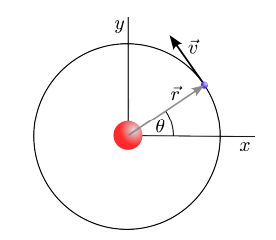
\includegraphics[width=0.6\textwidth]{images/quanten-hardware/Rotor.png}
    \caption{Schematische Darstellung eines Rotors nach Baumann (2024)}
    \label{fig:meinbild}
\end{figure}

Ein Laserstrahl mit passender Wellenlänge wird genutzt, um Übergänge zwischen diesen Zuständen zu induzieren. Liegt die Frequenz des Lasers genau im Resonanzbereich der Energiedifferenz der beiden Zustände, so kann das Ion durch sogenannte Rabi-Oszillationen in eine beliebige Superposition gebracht werden. Die Dynamik des Übergangs lässt sich mathematisch durch die Rabi-Frequenz \( \Omega \) beschreiben, welche sowohl von der Intensität des Lasers als auch von der Stärke des Dipolmoments des Übergangs abhängt.

Die Kontrolle über Pulsdauer, Polarisation und Phase erlaubt die Realisierung verschiedener logischer Operationen wie beispielsweise das Hadamard-Gatter oder das Pauli-\( X \)-Gatter. Visualisiert wird der Zustand eines Qubits in der Praxis häufig durch die sogenannte Bloch-Kugel, in welcher jede mögliche Superposition von \( \lvert 0 \rangle \) und \( \lvert 1 \rangle \) einem Punkt auf der Kugeloberfläche entspricht.

Im Experiment werden zur Umsetzung meist extrem präzise, kurze Laserpulse verwendet, die eine hohe Adressiergenauigkeit einzelner Ionen gewährleistet (Baumann, 2024).

\subsubsection{Zwei-Qubit-Gatter}

Zwei-Qubit-Gatter ermöglichen es, Korrelationen zwischen Qubits herzustellen und bilden zusammen mit Ein-Qubit-Gattern eine universelle Menge an logischen Operationen. Die wohl bekannteste Zwei-Qubit-Operation ist das bereits vorgestellte CNOT-Gatter (Controlled-NOT-Gatter), das auf zwei Qubits wirkt: ein Kontroll- und ein Ziel-Qubit. Ist das Kontroll-Qubit im Zustand \( \lvert 1 \rangle \), wird ein NOT-Gatter auf das Ziel-Qubit angewendet; andernfalls bleibt es unverändert. Diese logische Verknüpfung bildet die Grundlage für viele quantenlogische Algorithmen und Verschlüsselungsverfahren.

In Ionenfallen wird ein solches Gatter durch die gemeinsame Kopplung der Ionen an die quantisierten Schwingungsmoden realisiert. Dabei dienen diese kollektiven Moden als ein „Phonon-Bus“, über den Zustände zwischen den Ionen ausgetauscht werden können (Baumann, 2025).

Zu den bedeutendsten realisierten Zwei-Qubit-Gattermodellen gehört das Cirac-Zoller- und das Mølmer-Sørensen-Gatter, welche im folgenden Abschnitt vorgestellt werden:

\newpage
\textbf{Cirac-Zoller-Gatter} 

Das von Cirac und Zoller im Jahr 1995 vorgeschlagene Gatter gilt als eines der ersten theoretisch und experimentell realisierten Modelle für ein entanglierendes Zwei-Qubit-Gatter in Ionenfallen. Hierbei wird ein drittes, sogenanntes Bus-Qubit über gezielte Laserpulse angeregt und zwischen zwei speichernden Ionen als Vermittler genutzt. Die Gatteroperation nutzt eine präzise definierte Sequenz aus Resonanzanregungen und kontrollierten Phasenverschiebungen, um über den Schwingungszustand gezielt einen Quantenbit-Zustand auf das andere zu übertragen.

Der Zustand \( \lvert 0 \rangle \lvert 1 \rangle \) kann beispielsweise durch das Gatter in eine Überlagerung mit \( \lvert 1 \rangle \lvert 0 \rangle \) überführt werden, wobei die Phononen nur temporär real angeregt werden. Die präzise Steuerung der Frequenzdifferenz, Laserstärke und Phasenlage ist essenziell. In der Praxis ist die Methode allerdings experimentell aufwendig, da sie eine sehr hohe Kontrolle über den Grundzustand der Ionen erfordert. Dennoch wurde sie erfolgreich in Experimenten mit Kalziumionen demonstriert(Cirac and Zoller, 1995; Baumann, 2025). 

\textbf{Mølmer-Sørensen-Gatter} 


Das Mølmer-Sørensen-Gatter (MS-Gatter) ist eine Weiterentwicklung, die sich in modernen Ionenfallen-Architekturen durchgesetzt hat. Anders als das Cirac-Zoller-Gatter benötigt es kein Bus-Qubit, sondern nutzt kollektive Schwingungsmoden zur gleichzeitigen Adressierung mehrerer Qubits.

Ein typisches MS-Gatter basiert auf einem bichromatischen Laserpuls, welcher symmetrisch zwei Seitenbänder ober- und unterhalb der Qubit-Resonanzfrequenz anspricht. Dabei wird die Schwingung nur virtuell angeregt, was die Robustheit gegenüber thermischen Zuständen erhöht. Durch diese Wechselwirkung entsteht eine effektive Spin-Spin-Kopplung, mit der sich verschränkte Zustände, wie z.\,B. Bell-Zustände, effizient erzeugen lassen. Das Gatter benötigt dabei nur minimale Kontrolle über die Bewegungszustände der Ionen, was es besonders fehlerresistent und skalierbar macht. Zudem kann es gleichzeitig mehrere Qubit-Paare verschränken (Mølmer and Sørensen, 2000; Baumann, 2025).

\begin{table}[ht]
    \centering
    \caption{Vergleich zwischen Cirac-Zoller- und Mølmer-Sørensen-Gatter WIP}
    \label{tab:vergleich_gatter}
    \begin{tabular}{p{4.5cm} p{5.5cm} p{5.5cm}}
        \textbf{Eigenschaft} & \textbf{Cirac-Zoller-Gatter} & \textbf{Mølmer-Sørensen-Gatter} \\
        Jahr & 1995 & ~2000 \\
        Vermittlung & Bus-Qubit notwendig & Keine zusätzlichen Qubits \\
        Schwingungsmoden & Echt angeregt & Virtuell angeregt \\
        Robustheit & Gering (gegenüber thermischen Zuständen) & Hoch \\
        Skalierbarkeit & Eingeschränkt & Gut skalierbar \\
        Experimentelle Anforderungen & Hohe Präzision & Weniger streng \\
        Anwendungsbereich & Proof-of-Concept & Industrielle Prototypen \\
    \end{tabular}
\end{table}


\subsection{Aufbau und Betriebsweise eines Ionenfallencomputers}

Während theoretische Betrachtungen von Ionenfallen-Qubits sich stark auf die physikalischen Prinzipien konzentrieren, wie in Abschnitt 1.6.3 beschrieben, unterscheidet sich der tatsächliche Aufbau eines Ionenfallen-Quantencomputers in der Praxis erheblich durch seine technische Komplexität. Moderne Systeme verbinden physikalisch hochpräzise Komponenten mit klassischer Computertechnik und Softwareintegration, welche im folgenden Kapitel genauer vorgestellt werden.
\subsubsection{Beispiele in Reale Systemen}

Ein anschauliches Beispiel für die Realisierung eines kommerziellen Ionenfallen-Quantencomputers liefert das österreichische Unternehmen Alpine Quantum Technologies (AQT). Der Quantenprozessor von AQT ist vollständig in ein standardisiertes 19-Zoll-Gehäuse integriert, das äußerlich kaum von einem klassischen Serverschrank unterscheidbar ist. Im Inneren befinden sich jedoch Hochvakuumkammern, mikrostrukturierte Paul-Fallen, Lasermodule, modulare Optiksysteme und eine komplexe Steuerungseinheit. Die Quantenhardware wird durch klassische Komponenten ergänzt, die für Temperaturkontrolle, Impulssteuerung, Datenausgabe und externe Kommunikation zuständig sind (Bischoff et al., 2024).

    \begin{figure}[ht]
    \centering
    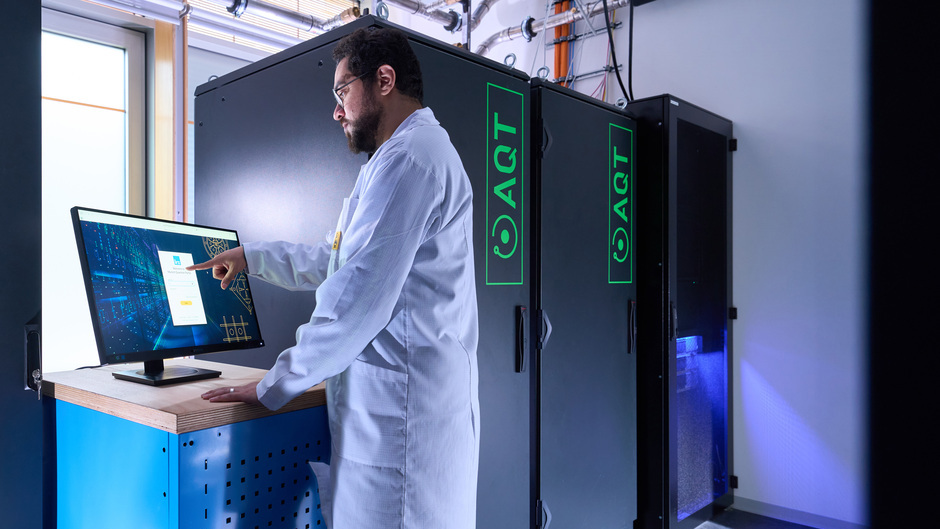
\includegraphics[width=1\textwidth]{images/quanten-hardware/AQT.jpg}
    \caption{Bild eines AQT Ionenfallencomputers}
    \label{fig:meinbild}
    \end{figure}

AQT entwickelt seine Systeme auf der Grundlage langjähriger Forschung an der Universität Innsbruck, insbesondere in Kooperation mit dem Experimentalphysiker Rainer Blatt, Mitgründer von AQT, der als einer der Pioniere der Ionenfallenplattform gilt (Blatt and Wineland, 2008). Die Geräte verwenden typischerweise linear angeordnete Ionenketten aus Kalziumionen, die in einer mikrochip-basierten Paul-Falle fixiert werden. Diese Chips sind modular aufgebaut und lassen sich bei Bedarf austauschen oder erweitern. Die Laseransteuerung, die Ioneninitialisierung, das Auslesen der Zustände und die zeitlich exakte Koordination der Gatteroperationen erfolgen über eine integrierte Steuerelektronik, meist in Form von FPGA-gestützter Signalverarbeitung .

Auch andere Systeme wie Quantinuum (ehemals Honeywell Quantum) oder IonQ verfolgen vergleichbare Ansätze: Der eigentliche Quantenprozessor wird in eine vollständig abgeschirmte Umgebung eingebettet, kombiniert mit photonischer Signalverarbeitung und einem modularen optischen Kontrollsystem. So wurde etwa 2024 an der Universität Innsbruck erstmals eine Verschränkung von 56 Ionen auf einem einzigen Chip demonstriert, ein Rekord für die Ionenfallenplattform (Bischoff et al., 2024). 

Neben AQT existieren heute weltweit mehrere Firmen, die Ionenfallen-Quantencomputer entwickeln oder bereits kommerziell anbieten, darunter eQtron in Siegen, Universal Quantum in Sussex, IonQ in Maryland (USA) sowie Quantumium in Colorado. 
Trotz des unterschiedlichen Designs verfolgen alle diese Plattformen einen ähnlichen Architekturansatz: Die Trennung von quantenphysikalischem Kernsystem (Ionenchip, Lasermodule, Vakuum) und klassischer Steuerungseinheit, die die Verbindung zur Außenwelt und Benutzersteuerung herstellt. Diese einzelnen Komponenten werden in den nächsten Kapiteln genauer erläutert.

\subsubsection{Quantenarchitekturen von Ionenfallencomputern}
Die genaue Funktionsweise eines Ionenfallen-Quantencomputers, also die Architektur, beschreibt das physikalische und logische Zusammenspiel seiner Komponenten – insbesondere, wie Ionen gespeichert, bewegt und miteinander verschränkt werden. Während erste Systeme auf starren linearen Anordnungen basierten, sind moderne Architekturen zunehmend modular, rekonfigurierbar und auf Skalierbarkeit ausgelegt. Es lassen sich grundlegende Architekturen unterscheiden, die in der Praxis aktuell Anwendung finden.
\\\\
\paragraph{Paul-Falle}

Die bekannteste Realisierungsform stellt die lineare Paul-Falle dar, wie sie beispielsweise von AQT verwendet wird \cite{bischoff2024}. Diese wurde im vorherigen Kapitel bereits vorgestellt. AQT hält die Ionen in einer eindimensionalen Kette, wobei eine X-förmige Elektrodengeometrie hohe Fallenfrequenzen bei gleichzeitig guter optischer Zugänglichkeit ermöglicht \cite{frisch2024, strohm2024}. In diesen sogenannten Surface Traps erlaubt die Chip-Architektur die präzise Adressierung einzelner Ionen sowie das Auslesen durch seitlich einfallende Laserstrahlen, um Gatteroperationen auszuführen \cite{strohm2024}.

\medskip

\paragraph{QCCD-Architektur}

Eine skalierbare Architektur ist das sogenannte \textit{Quantum Charge-Coupled Device} (QCCD), das 2002 von Kielpinski et al.\ erstmals vorgestellt wurde \cite{kielpinski2002}. Sie basiert auf der Trennung von Rechen-, Speicher- und Transportzonen. In dieser Architektur, wie sie beispielsweise von Quantinuum verfolgt wird, werden Ionen gezielt zwischen verschiedenen Zonen bewegt, um dort Gatteroperationen auszuführen oder für spätere Nutzung zu speichern. Um diese Parallelisierung zu ermöglichen, muss die Architektur folgende Anforderungen erfüllen: schnelle und verlustarme Transporte, Synchronisation über viele Kontrollzonen, Phasenstabilität sowie ggf. die Kombination unterschiedlicher Ionenarten zur Kühlung \cite{strohm2024}.

\medskip

\paragraph{Race-Track-Architektur}

Ein alternativer Vorschlag zur QCCD-Struktur ist die sogenannte \textit{Race-Track-Architektur}. Dabei handelt es sich um eine ringförmige Anordnung von Rechen- und Speicherzonen, die einer Rennbahn ähneln. In aktiven Zonen finden dabei Gatteroperationen statt, während ruhende Ionen in den sogenannten Parking-Zonen mit optimierter Kohärenzzeit gelagert werden. Dieses Layout erlaubt eine fortlaufende Umverteilung der Ionen bei gleichzeitig geringer Kreuzkopplung zwischen den Operationen und minimierter Störanfälligkeit \cite{strohm2024}.

\medskip

\paragraph{Photonische Interkonnekte}

Ein weiterer Schritt zur Skalierung über die Chipgrenzen hinaus besteht in der Verbindung mehrerer Ionenfallenmodule über photonische Interkonnekte. Hierbei werden einzelne Ionen über Lichtteilchen (Photonen) miteinander verschränkt, die durch Faseroptiksysteme aus zwei verschiedenen Fallen in einen Strahlteiler gelenkt und dort überlagert werden \cite{strohm2024}. Dieser als photon-mediated entanglement bekannte Mechanismus erlaubt es, logische Qubits über große Distanzen hinweg zu koppeln, beispielsweise im Rahmen verteilter Quantenrechner \cite{strohm2024}.
\\\\
Wie die vorgestellten Architekturen verdeutlichen, stellt insbesondere die Skalierung eine zentrale Herausforderung bei der Weiterentwicklung von Ionenfallen-Quantencomputern dar – ein Aspekt, der in Kapitel (Insert Kapitel) vertiefend im Kontext der technischen Limitationen behandelt wird.

\subsubsection{Hardwareinfrastruktur von Ionenfallencomputern}
Jede Quantenarchitektur ist abhängig von ihrer eingebauten Hardwareinfrastruktur innerhalb eines Ionenfallen-Quantencomputers und stellt gleichzeitig ein hochkomplexes Zusammenspiel verschiedener Subsysteme dar. Um den stabilen Betrieb zu gewährleisten, müssen zahlreiche technische Anforderungen erfüllt werden. Die folgenden Abschnitte beleuchten die zentralen Komponenten im Überblick: \\

\textbf{Vakuum- und Kühlungstechnik} \\
Eine der zentralen Voraussetzungen für den stabilen Betrieb von Ionenfallen-Quantencomputern ist ein Ultrahochvakuum (UHV) mit Drücken im Bereich von etwa $10^{-11}$~Torr. Bereits einzelne Kollisionen mit Restgasmolekülen – etwa Wasserstoff – können zu Qubit-Verlust, Ionenketten-Umsortierung oder vollständigem Herausfallen aus der Falle führen. Daher müssen Störungen durch Gasmoleküle nahezu vollständig ausgeschlossen werden \cite{ionq2025}. \\
Aikyo et al.\ \cite{aikyo2020} beschreiben, dass die Qualität des Vakuums nicht nur durch direkte Messung, sondern auch experimentell über Beobachtungen von z.\,B.\ Ketten-Rekonfigurationen quantifiziert wurde. Diese erlauben Rückschlüsse auf die effektive Kollisionsrate mit Hintergrundgas – typischerweise ein Ereignis alle 16 bis 30 Minuten –, was für stabile Quantengatter ausreichend ist. Die mittlere freie Weglänge eines Moleküls im UHV beträgt mehrere tausend Kilometer, im Vergleich zu wenigen Nanometern bei Normaldruck. \\
Alternativ nutzen manche Anbieter kryogene Kühlung, um bei tiefen Temperaturen (< 12 K) eine noch höhere Vakuumqualität zu erreichen. Bei solchen Temperaturen fungieren kalte Oberflächen zusätzlich als effektive Getterflächen und verringern die Heizrate der Ionen. \\
Die Vakuum- und Kühlungstechnik ist somit nicht nur passives Mittel zur Isolation, sondern ein integraler Bestandteil der Qubit-Lebensdauer, Gate-Fidelity und Skalierbarkeit von Ionenfallen-basierten Quantencomputern. \\

\textbf{Optische Systeme} \\
Optische Systeme übernehmen zentrale Aufgaben in der Strahlführung für Laserkühlung, Zustandsmanipulation und Messung. Laser werden meist extern erzeugt und über fasergekoppelte Optiken in die Nähe der Ionenfalle geleitet. Dort erfolgt die Fokussierung auf einzelne Ionen mithilfe von Hoch-NA-Objektiven oder mikrostrukturierten Linsenarrays. \\
Traditionell wird die Fluoreszenzdetektion bei Ionen mit Kameras, Photomultipliern oder Avalanche-Photodioden durchgeführt. Neuerdings kommen jedoch auch CMOS-kompatible Einzelphotonen-Avalanchedioden zum Einsatz, welche bei Raumtemperatur betrieben werden können und für spezifische Wellenlängen optimiert sind. In Kombination mit mikrostrukturierten Fresnel-Zonenplatten lassen sich so kompakte Detektionssysteme realisieren, die skalierbar sind und sich auch für Ionenfallen eignen \cite{chatterjee2023}. \\

\textbf{Steuerungselektronik} \\
Die Steuerungselektronik stellt das zentrale Bindeglied zwischen Quantenhardware und klassischer Kontrolle dar. Sie umfasst alle Systeme zur Erzeugung und Modulation von Spannungen, Frequenzen und Pulsen, die zum Betrieb der Falle, zur Qubit-Manipulation und für Messprozesse erforderlich sind. Moderne Ionenfallen-Quantencomputer verwenden hierzu hochpräzise FPGA-basierte Sequenzcontroller in Kombination mit digitaler Signalverarbeitung (DSP) direkt auf Hardwareebene \cite{keysight2024}. \\
Für die Lasersteuerung kommen modulierte Signale zum Einsatz, die über Acousto-Optic Modulatoren (AOMs) und Electro-Optic Modulatoren (EOMs) kontrolliert werden. Diese modulieren Frequenz, Phase und Intensität der Laserstrahlen präzise. Die Steuerung dieser Modulatoren erfolgt typischerweise über Arbitrary Waveform Generators (AWGs) mit FPGA-Unterstützung, die flexible Pulsgestaltung, Echtzeit-Phasenkontrolle und latenzoptimierte Parameter-Scans erlauben \cite{keysight2024}. \\
Auch Mikrowellenquellen spielen eine Rolle, insbesondere bei Qubits mit Hyperfeinübergängen. Diese dienen nicht nur als Ansteuerung für direkte Rotationen, sondern auch als Lokaloszillatoren in Kombination mit optischen Trägern \cite{keysight2024}. \\

Die vorgestellten Subsysteme bilden das technologische Rückgrat ionenbasierter Quantencomputer. Dabei entscheidet nicht nur die Wahl der physikalischen Komponenten über die Leistungsfähigkeit des Systems – auch ihre Integration und Synchronisation sind entscheidend für die spätere Nutzung.

\subsubsection{Anwendungen mit Ionenfallencomputern}
Trotz der noch begrenzten Qubit-Zahlen konnten Ionenfallen-Quantencomputer bereits erfolgreich in verschiedenen Bereichen praktisch erprobt werden. Der Vorteil dieser Plattform liegt insbesondere in ihren hardwarebedingten Stärken: hohe Gatterfidelitäten, lange Kohärenzzeiten sowie eine flexible All-to-All-Konnektivität, wodurch viele Algorithmen besonders effizient umgesetzt werden können \cite{strohm2024}. \\

In den letzten Jahren wurden reale Ionenfallensysteme u.\,a.\ für chemische Simulationen (etwa von Molekülen wie H\textsubscript{2}O oder LiH), kombinatorische Optimierungsprobleme (z.\,B.\ MaxCut mittels QAOA) sowie Ansätze im Quantum Machine Learning genutzt. Hierbei konnten trotz begrenzter physischer Qubit-Zahl durch Reuse- und Zerlegungsmethoden auch größere Probleme adressiert werden \cite{strohm2024}. \\

Mehrere vorgestellte Unternehmen stellen ihre Systeme bereits Forschungs- und Industriepartnern zur Verfügung. Damit bilden Ionenfallen-Quantencomputer schon heute eine Plattform mit unmittelbarem Anwendungspotenzial. Eine vertiefte Betrachtung konkreter Anwendungsfelder in Chemie, Medizin, Industrie und Finanzwesen erfolgt in den Kapiteln~7 bis~10.

\subsection{Herausforderungen und technische Limitationen}
\subsubsection{Herausforderung bei der Skalierung}
Die Skalierung ist eine der zentralen Herausforderungen beim Bau großflächiger Ionenfallen-Quantencomputer. Während sich Ionen als nahezu identische und stabil manipulierbare Qubits eignen, stoßen heutige Architekturen bei mehr als 56~Qubits an technische Grenzen \cite{strohm2024, bischoff2024}. \\

Grundsätzlich lassen sich nach Strohm et al.\ \cite{strohm2024} zwei fundamentale Skalierungsprobleme in Ionenfallen identifizieren:
\begin{enumerate}
    \item Das \textit{Wiring-Problem} beschreibt die Schwierigkeit, jedem Qubit individuell steuerbare elektrische und optische Signale zuzuführen, insbesondere bei steigender Qubitanzahl. Je mehr Ionen adressierbar sein sollen, desto mehr digitale/analoge Kanäle, Laserlinien und Modulationspfade werden benötigt.
    \item Das \textit{Sorting-Problem} bezieht sich auf die Notwendigkeit, Qubits für Gatteroperationen physisch zueinander zu bewegen, da direkte Zwei-Qubit-Gatter in verschiedenen Fallenregionen nicht möglich sind.
\end{enumerate}

Ein wesentliches Hindernis ist der physikalische Aufbau linearer Paul-Fallen. In diesen Architekturen erhöht sich mit wachsender Ionenanzahl die Komplexität der Modenstruktur und die Anfälligkeit gegenüber Heizprozessen, was sich negativ auf die Gattertreue und Fehlerraten auswirkt. Zudem nimmt der Abstand der Ionen ab, was das gezielte Ansprechen einzelner Teilchen durch fokussierte Laserstrahlen erschwert. \\

Alternative Architekturen wie die vorgestellte QCCD-Struktur stellen eine bessere Option zur Hochskalierung dar, sind jedoch ebenfalls vom Wiring-Problem betroffen: Jeder Segmentbereich der Falle benötigt dedizierte Spannungs- und Taktsignale, wodurch die Anzahl der benötigten Leitungen stark ansteigt. Dies stellt hohe Anforderungen an das Packaging und die Steuerelektronik \cite{strohm2024}. \\

Auch das Sorting-Problem wird durch QCCD zwar strukturell adressiert, bleibt aber ein zeitkritischer Engpass. Denn das \textit{Shuttling}, also der physische Transport eines Ions über die Falle, verursacht zusätzliche Dekohärenz und verlängert die Gesamtausführungszeit eines Quantenprogramms. Strohm et al.\ \cite{strohm2024} berichten, dass der typische Zeitverbrauch in einem Algorithmus bei etwa 58\,\% für Transport, 41\,\% für Kühlung und nur 1\,\% für eigentliche Gatteroperationen liegt. Der Transport eines Ions über 200\,$\upmu$m dauert dabei rund 10\,$\upmu$s, was sich bei komplexen Programmen schnell aufsummiert. \\

\textbf{Lösungsansätze} \\
Zur Verbesserung der Skalierbarkeit von Ionenfallen-Quantencomputern wurden verschiedene Ansätze entwickelt, die sowohl auf der Hardware- als auch auf der Steuerungsebene ansetzen. Ein Schwerpunkt liegt auf der Optimierung der Ionentransporte: Effizientere Shuttling-Protokolle, etwa durch adiabatische Rampen oder fein segmentierte Steuerstrukturen, können unerwünschte Heizprozesse minimieren und gleichzeitig die Gatterfidelität bei bewegten Ionen verbessern. \\

Beim \textit{Qubit-Recycling} werden Ionen nach einer Zwischenauslesung durch schnelles Resetting erneut für Berechnungen genutzt. Dadurch lässt sich die effektive Anzahl nutzbarer Qubits erhöhen, ohne die physische Ionenanzahl zu vergrößern \cite{strohm2024}. \\

Auch der Einsatz sogenannter \textit{Qudits}, also Ionen, die mehr als zwei logisch adressierbare Energiezustände besitzen, kann zur Effizienzsteigerung beitragen. In ersten Experimenten wurden bereits achtstufige Qudits auf Basis von $^{40}\mathrm{Ca}^{+}$-Ionen realisiert. Diese erlauben native Qudit-Gatter, ohne dass die Systeme auf binäre Qubit-Logik beschränkt sind \cite{strohm2024}.

\subsubsection{Herausforderung bei Fehlertoleranz und Fehlerkorrektur}
Die Implementierung von fehlertoleranten Quantenoperationen ist eine weitere Herausforderung auf dem Weg zu skalierbaren und zuverlässigen Quantencomputern. Obwohl Ionenfallen-Systeme im Vergleich zu anderen Plattformen bereits von Natur aus über lange Kohärenzzeiten und hohe Gatterfidelitäten verfügen – 98{,}5\,\% bis 99{,}82\,\% bei Zwei-Qubit-Gattern \cite{strohm2024} –, reichen diese Werte für fehlerfreies Rechnen im großen Maßstab nicht aus. Daher ist der Einsatz von Quantenfehlertoleranz und Quantenfehlerkorrektur unverzichtbar. \\

Grundvoraussetzung für fehlertolerantes Quantencomputing ist die Möglichkeit, einen logischen Qubit-Zustand über mehrere physikalische Qubits hinweg so zu kodieren, dass Fehler erkannt und korrigiert werden können, ohne dabei den logischen Zustand selbst zu gefährden. Dazu müssen zunächst sogenannte Fehlerkorrekturcodes implementiert werden, wie etwa der \textit{Steane-Code}, bei dem ein logisches Qubit durch sieben physikalische Qubits repräsentiert wird. Entscheidend ist hierbei, dass sowohl die Initialisierung des logischen Zustands, die Messung potenzieller Fehler als auch die eigentliche Fehlerkorrektur selbst fehlertolerant durchgeführt werden, um keine weiteren Fehler in das System einzuführen \cite{strohm2024}. \\

Die technische Umsetzung dieser Konzepte bringt jedoch erhebliche Herausforderungen mit sich. Zum einen erfordert der Einsatz von Fehlerkorrekturverfahren einen hohen Qubit-Overhead: Für ein einziges logisches Qubit werden je nach Verfahren typischerweise sieben bis über hundert physikalische Qubits benötigt. Damit steigt nicht nur der Platzbedarf, sondern auch die Komplexität in der Steuerung und Kalibrierung exponentiell an. \\

Zum anderen ist die fehlerfreie und echtzeitfähige Messung von Syndromen technisch anspruchsvoll, da jede Messung selbst fehleranfällig ist und wiederum durch zusätzliche Kontrollqubits abgesichert werden muss. Hinzu kommen reale physikalische Fehlerquellen, die in heutigen Modellen oft nicht vollständig abgebildet sind – wie etwa positionsabhängiges Laserdetuning oder systematische Rauschquellen \cite{strohm2024}. \\

\textbf{Lösungsansätze} \\
Trotz dieser Herausforderungen wurden in Ionenfallen-Systemen bereits beachtliche Fortschritte erzielt. So konnte in mehreren Studien demonstriert werden, dass sich ein logisches Qubit erfolgreich gemäß dem Steane-Code kodieren lässt \cite{strohm2024}. Auch die fehlerresistente Messung von Fehler-Syndromen wurde erfolgreich mithilfe von \textit{Flag-Qubits} umgesetzt, die sogenannte \textit{Hook-Fehler} detektieren können – Fehler, die sich über Kontrollstrukturen auf Datenqubits ausbreiten würden. \\

Besonders hervorzuheben sind experimentelle Demonstrationen vollständiger Fehlerkorrekturzyklen, etwa für Phasenfehler in Drei-Ionen-Systemen oder für kombinierte Bit- und Phasenfehler im Rahmen des Sieben-Qubit-Steane-Codes. Darüber hinaus wurden erste logische Gatter auf Basis von \textit{Lattice Surgery} gezeigt, bei denen logische Qubits durch gezieltes Verschmelzen und Trennen von physikalischen Qubit-Verbänden verarbeitet werden \cite{strohm2024}.

\section{Quantencomputer auf Basis diamantbasierter Qubits (NV-Zentren)}
Dieses Kapitel widmet sich der Hardware-Implementierung von Quantencomputern, die auf Stickstoff-Fehlstellen-Zentren (NV-Zentren) in Diamant basieren. Diese spezifischen Defekte im Diamantgitter bieten eine vielversprechende Plattform für Qubits, insbesondere aufgrund ihrer Fähigkeit, bei Raumtemperatur zu funktionieren. QUELLE1 Wir werden zunächst die physikalischen Grundlagen dieser diamantbasierten Qubits beleuchten, gefolgt von der Implementierung von Quantengattern. Anschließend werden die verschiedenen Verwendungsbereiche und Merkmale dieser Technologie sowie die aktuellen Herausforderungen und Limitationen diskutiert.
\subsection{Physikalisches Prinzip}
\subsubsection{Das Zwei-Niveau-System: Elektronenspins von Stickstoff-Fehlstellen (NV-Zentren) im Diamantgitter}
Ein Stickstoff-Fehlstellen-Zentrum, kurz NV-Zentrum (vom Englischen Nitrogen-Vacancy), ist eine spezifische atomare Störung in der perfekten Kohlenstoffstruktur des Diamanten. QUELLE1 Es entsteht, wenn ein Kohlenstoffatom durch ein Stickstoffatom ersetzt wird und ein benachbarter Gitterplatz leer bleibt – eine sogenannte Vakanz oder Fehlstelle. QUELLE1 In diesem Defekt werden Elektronen eingefangen, und es ist der Spin dieser Elektronen, der als Qubit genutzt wird. QUELLE1 Für Quantenanwendungen werden häufig synthetische Diamanten verwendet, da bei ihrer Herstellung Stickstoffatome gezielt in das Kristallgitter eingebracht werden können, um die gewünschten NV-Zentren zu erzeugen. QUELLE1
Der elektronische Grundzustand eines NV-Zentrums ist ein sogenannter Triplett-Zustand, der drei mögliche Spinzustände aufweist: m s = 0, m s = +1 und m s = -1. QUELLE1 Ohne ein äußeres Magnetfeld haben die Zustände m s = +1 und m s = -1 die gleiche Energie (sie sind entartet), während der Zustand m s = 0 energetisch von ihnen getrennt ist. Diese Energietrennung, die sogenannte Nullfeldaufspaltung, beträgt etwa 2,87 bis 2,88 GHz. QUELLE1
Um ein Qubit zu bilden, wählt man aus diesen drei Spinzuständen zwei als Basiszustände für das Zwei-Niveau-System aus. Beispielsweise könnte der m s = 0 Zustand als |0⟩ und die entarteten m s = ±1 Zustände als |1⟩ definiert werden. QUELLE1 Durch Anlegen eines äußeren Magnetfeldes kann die Entartung der m s = ±1 Zustände aufgehoben werden (Zeeman-Effekt), wodurch man zwei voneinander getrennte Energieniveaus erhält, die dann als |0⟩ und |1⟩ dienen können. QUELLE1 Obwohl das NV-Zentrum ein komplexeres System mit mehreren Energieniveaus ist, wird es durch die gezielte Ansteuerung von nur zwei dieser Zustände effektiv zu einem Zwei-Niveau-System, das als Qubit für die Quanteninformationsverarbeitung genutzt werden kann. QUELLE3
\subsubsection{Optische Kontrolle von NV-Qubits}
Die optische Kontrolle ist ein grundlegender Mechanismus zur Interaktion mit NV-Qubits. Sie dient hauptsächlich dazu, das Qubit in einen bekannten Ausgangszustand zu bringen (Spin-Initialisierung) und seinen Endzustand nach einer Operation auszulesen. QUELLE1 Dies geschieht typischerweise durch Bestrahlung mit grünem Laserlicht, das das NV-Zentrum von seinem elektronischen Grundzustand (³A) in einen angeregten Zustand (³E) anhebt. QUELLE1
Der Ausleseprozess basiert auf der Fluoreszenz des NV-Zentrums. Der angeregte Zustand kann auf verschiedene Weisen in den Grundzustand zurückfallen, wobei ein Teil des Zerfalls über einen metastabilen Singulett-Zustand (¹A) verläuft. QUELLE1 Entscheidend ist, dass die Intensität des emittierten Lichts (Fluoreszenz) vom jeweiligen Elektronenspinzustand abhängt. Beispielsweise fluoresziert der m s = 0 Zustand in der Regel heller als die m s = ±1 Zustände. QUELLE1 Durch Messen der Menge des emittierten Lichts kann somit auf den Spinzustand des Qubits geschlossen werden. QUELLE1 Eine charakteristische optische Signatur des negativ geladenen NV-Zentrums ([NV]$^{-}$) ist die sogenannte Null-Phononen-Linie (ZPL) bei 638 nm, die eine eindeutige Identifizierung und Charakterisierung ermöglicht. QUELLE1
Die Fähigkeit des Elektronenspins im NV-Zentrum, mit Photonen (Lichtteilchen) zu interagieren, ist von großer Bedeutung. Diese Wechselwirkung schafft eine natürliche Schnittstelle zwischen stationären Qubits im Diamanten und "fliegenden" Qubits in Form von Photonen. QUELLE1 Diese Wechselwirkung ermöglicht es, Quantenzustände über weite Strecken zu übertragen und NV-Zentren miteinander zu verbinden und zu verschränken, was für den Aufbau skalierbarer Quantensysteme entscheidend ist. QUELLE3
\subsubsection{Mikrowellensteuerung von NV-Qubits}
Während optische Methoden ideal für die Initialisierung und das Auslesen von NV-Qubits sind, erfolgt die präzise Manipulation des Spinzustands – also die Durchführung von Quantenoperationen oder "Gattern" – typischerweise mithilfe von Mikrowellenstrahlung.QUELLE1 Mikrowellen nutzen die bereits erwähnte Energieaufspaltung zwischen dem m s = 0 und den m s = ±1 Zuständen des Elektronenspins. Durch Anlegen von Mikrowellenpulsen bei der Resonanzfrequenz (um 2,87 GHz) können kohärente Übergänge zwischen diesen Spinzuständen gezielt angeregt werden. QUELLE1 Dieses Prinzip bildet die Grundlage der optisch detektierten magnetischen Resonanz (ODMR), einer Schlüsseltechnik zur Untersuchung und Kontrolle von NV-Zentren. QUELLE1
Zusätzlich können externe Magnetfelder angelegt werden, um die m s = ±1 Zustände weiter aufzuspalten (Zeeman-Effekt). Dies ermöglicht eine noch präzisere Kontrolle und Adressierung einzelner Spinzustände. QUELLE1 Die kohärente Manipulation des Qubit-Zustands mittels Mikrowellen ist entscheidend für die Ausführung von Quantenalgorithmen, da sie die Erzeugung und Kontrolle beliebiger Superpositionen und Verschränkungen erlaubt. QUELLE3
Die Kombination aus optischer und Mikrowellensteuerung bietet ein vollständiges Instrumentarium zur Handhabung von NV-Qubits. Die optische Kontrolle ist effizient für die Vorbereitung des Qubits in einem bekannten Zustand und das Auslesen von Informationen, während die Mikrowellensteuerung die für kohärente Quantenoperationen (Gatter) erforderliche Präzision liefert. QUELLE3
\subsection{Gatterimplementierung}
    - Ein-Qubit-Gatter
    - Zwei-Qubit-Gatter
\subsection{Verwendungsbereiche und Merkmale der diamantbasierten Qubits}
    - Stand der Technologie
    - Anwendungen
    - Systemaufbau
    - Betriebsbedingungen
\subsection{Herausforderungen und technische Limitationen}
    - Warum gibt es die aktuellen Probleme?
    - Skalierbarkeit
    - Gatterzeiten:
    - Potenzial und Ansätze:


% \addbibressource{content/jakob/citations.bib}

\section{Photonen und andere Ansätze}
Die Realisierung eines skalierbaren, fehlertoleranten Quantencomputers stellt eine der größten wissenschaftlichen und technischen Herausforderungen unserer Zeit dar (\cite{QuantumHardwareExplained}). Weltweit werden diverse physikalische Systeme intensiv erforscht, um die komplexen Anforderungen an Quantenhardware zu erfüllen (\cite{chengNoisyIntermediatescaleQuantum2023}). Diese Vielfalt an Ansätzen spiegelt die Tatsache wider, dass noch kein einzelnes System alle notwendigen Kriterien optimal erfüllt und der Weg zu universellen Quantencomputern nicht singulär erscheint. Vielmehr deutet die aktuelle Forschungslandschaft auf eine längere Phase paralleler Entwicklungen und potenzieller Hybridisierungen hin, in der verschiedene Technologien koexistieren und möglicherweise integriert werden, anstatt dass eine einzelne Technologie die anderen schnell verdrängt (\cite{QuantumHardwareExplained}).
\newline \newline
Ein etablierter Rahmen zur Bewertung der verschiedenen Hardwareplattformen sind die DiVincenzo-Kriterien (\cite{QuantumComputingArchitecture}). Diese umfassen typischerweise die Existenz gut charakterisierter Qubits, die Möglichkeit zur Initialisierung der Qubits in einen definierten Zustand, lange Kohärenzzeiten, die Fähigkeit zur Durchführung universeller Quantengatter sowie eine zuverlässige Auslesemethode für Qubits. Die Erfüllung dieser Kriterien unterliegt signifikanten ingenieurtechnischen Hürden, die Expertise aus Physik, Kryotechnik, Materialwissenschaften und Elektronik erfordern (\cite{QuantumHardwareExplained}).
\newline \newline
Dieses Kapitel fokussiert auf photonische Quantencomputer als einen prominenten alternativen Ansatz und beleuchtet darüber hinaus weitere vielversprechende Technologien wie Halbleiter-Spin-Qubits und topologische Qubits. Es wird anerkannt, dass etabliertere Plattformen wie supraleitende Qubits (\cite{QuantumComputingArchitecture}) und gefangene Ionen (\cite{sruthisomarouthuQuantumComputingDigital2025}) bereits einen höheren Reifegrad erreicht haben und vermutlich in anderen Kapiteln dieses Buches ausführlich behandelt werden. Die hier diskutierten Ansätze zeichnen sich durch spezifische Vorteile und innovative Lösungsstrategien für die Kernprobleme der Quanteninformationsverarbeitung aus.
\newline \newline
Die aktuelle Ära der Quantencomputerentwicklung wird häufig als „Noisy \linebreak Intermediate-Scale Quantum“ (NISQ) bezeichnet (\cite{chengNoisyIntermediatescaleQuantum2023}). In dieser Phase sind die verfügbaren Quantenprozessoren noch fehleranfällig und die Anzahl der Qubits begrenzt. Ein zentrales Forschungsziel ist daher die Entwicklung und Implementierung von Strategien zur Fehlerminderung und -korrektur sowie die Realisierung sogenannter logischer Qubits, die eine höhere Robustheit gegenüber physikalischen Fehlern aufweisen (\cite{QuantumHardwareExplained}). Dieser Trend zur Fehlertoleranz ist ein kritisches Moment in der Entwicklung und signalisiert eine Verschiebung von der reinen Demonstration quantenmechanischer Phänomene hin zur Bewältigung der ingenieurtechnischen Herausforderungen für praktische Quantenvorteile. Jede Bewertung der hier vorgestellten „anderen Ansätze“ muss daher nicht nur die rohe Qubit-Anzahl, sondern auch den Fortschritt und die Strategien auf dem Weg zur Fehlertoleranz berücksichtigen.

\subsection{Photonische Quantencomputer}
Photonische Quantencomputer nutzen Lichtquanten (Photonen) als Träger von Quanteninformation. Dieser Ansatz bietet eine Reihe einzigartiger Vorteile, steht aber auch vor spezifischen Herausforderungen, die intensive Forschungs- und Entwicklungsanstrengungen erfordern.

\subsubsection{Grundlegende Prinzipien und Qubit-Kodierung}
Photonen werden oft als „fliegende Qubits“ bezeichnet, da sie sich naturgemäß mit Lichtgeschwindigkeit bewegen, eine geringe Wechselwirkung mit ihrer Umgebung aufweisen (was zu langer Kohärenz führt) und potenziell bei Raumtemperatur betrieben werden können (\cite{abughanemPhotonicQuantumComputers2024}). Die Kodierung von Qubits in Photonen kann auf verschiedene Weisen erfolgen. Eine verbreitete Methode ist die Dual-Rail-Kodierung, bei der die Zustände $\ket{0}$ und $\ket{1}$ durch die Anwesenheit eines Photons in einem von zwei räumlichen Moden (z. B. zwei Wellenleitern) oder zwei orthogonalen Polarisationen repräsentiert werden (\cite{slussarenkoPhotonicQuantumInformation2019}). Alternativ werden kontinuierliche Variablen (Continuous Variable, CV) Ansätze verfolgt, bei denen Qubits beispielsweise in gequetschten Lichtzuständen (Squeezed States) kodiert werden, wie es von Unternehmen wie Xanadu erforscht wird (\cite{QuantumComputingArchitecture}). Auch die Zeitmultiplex-Kodierung (Time-Bin Encoding), bei der die Ankunftszeit eines Photons relativ zu einem Referenzpuls das Qubit definiert, ist eine gängige Methode \cite{LinearOpticsScalable}.

\subsubsection{Schlüsselkomponenten}
Die Realisierung photonischer Quantencomputer hängt von drei Schlüsselkomponenten ab:
\par Photonenquellen: Eine Herausforderung ist die Erzeugung einzelner Photonen bei Bedarf (deterministisch). Probabilistische Quellen, basierend auf spontaner parametrischer Fluoreszenz (Spontaneous Parametric Downconversion, SPDC), sind zwar etabliert, aber für skalierbare Systeme ineffizient (\cite{slussarenkoPhotonicQuantumInformation2019}). Daher liegt ein starker Fokus auf der Entwicklung deterministischer oder angekündigter (heralded) Einzelphotonenquellen, beispielsweise basierend auf Quantenpunkten (\cite{LinearOpticsScalable}) oder Halbleiter-Quantenemittern, wie sie Quandela einsetzt (\cite{QuandelaAnnounces100000fold2025}). Kürzlich wurde über Quantenpunktquellen mit Helligkeiten über 106 Photonenpaaren/s/mW und angekündigte Einzelphotonenquellen mit Reinheiten über 99\% berichtet (\cite{LinearOpticsScalable}).
\par Manipulation: Die Manipulation photonischer Qubits erfolgt durch lineare optische Elemente wie Strahlteiler und Phasenschieber (\cite{slussarenkoPhotonicQuantumInformation2019}). Für erhöhte Stabilität, Miniaturisierung und Skalierbarkeit werden zunehmend integrierte photonische Schaltkreise (Photonic Integrated Circuits, PICs) eingesetzt (\cite{abughanemPhotonicQuantumComputers2024}). Diese PICs werden auf verschiedenen Materialplattformen wie Silizium, Siliziumnitrid oder Lithiumniobat realisiert.
\par Detektion: Hocheffiziente Einzelphotonendetektoren sind unerlässlich. Supraleitende Nanodraht-Einzelphotonendetektoren (Superconducting Nanowire Single-Photon Detectors, SNSPDs) erreichen Detektionseffizienzen von über 98\% (\cite{LinearOpticsScalable}), stellen aber hohe Anforderungen an die Kühlung. Eine Herausforderung bleibt die photonenzahlauflösende Detektion (\cite{slussarenkoPhotonicQuantumInformation2019}).

\subsubsection{Vorteile und spezifische Herausforderungen}

Photonische Quantencomputer bieten eine Reihe signifikanter Vorteile. Ein wesentlicher Pluspunkt ist ihr Potenzial für den Raumtemperaturbetrieb bei einigen Komponenten, auch wenn Quellen und Detektoren oft eine Kühlung erfordern (\cite{abughanemPhotonicQuantumComputers2024}). Ferner zeichnen sich photonische Qubits durch eine geringe Dekohärenz aus, bedingt durch die schwache Wechselwirkung von Photonen mit ihrer Umgebung, was zu langen Kohärenzzeiten führt (\cite{abughanemPhotonicQuantumComputers2024}). Darüber hinaus eignen sich Photonen hervorragend für die Quantenkommunikation und -netzwerke, da sie als natürliche Informationsträger über lange Distanzen fungieren (\cite{abughanemPhotonicQuantumComputers2024}). Diese Eigenschaft positioniert die Photonik einzigartig für modulare Architekturen, bei denen spezialisierte photonische Module andere Arten von Quantenprozessoren miteinander verbinden und somit als „Quanten-Internet-Backbone“ dienen könnten.
\newline
\newline
Dem gegenüber stehen die spezifischen Herausforderungen Photonenverlust, probabilistische Qubit-Gatter und die Skalierbarkeit von Quellen, sowie Detektoren.
\par 
Photonenverlust: 
Dies ist ein Hauptproblem, das alle Komponenten betrifft – von der Quelle über die Manipulation bis zur Detektion – und die Fidelität stark beeinträchtigt (\cite{LinearOpticsScalable}). Strategien zur Minderung umfassen die Entwicklung von Materialien mit extrem geringen Verlusten (z. B. Siliziumnitrid) und die Verbesserung der Effizienz von Komponenten und Kopplungen (\cite{salavrakosPhotonnativeQuantumAlgorithms2025}).

\par Probabilistische Zwei-Qubit-Gatter:
Die schwache native Wechselwirkung zwischen Photonen macht deterministische Zwei-Qubit-Gatter sehr schwierig (\cite{slussarenkoPhotonicQuantumInformation2019}). Übliche Ansätze basieren auf messungsinduzierter Nichtlinearität unter Verwendung von Hilfsphotonen und Postselektion, was zu einem hohen Ressourcenaufwand führt. Alternative Ansätze wie Cluster-Zustands-basiertes oder fusionsbasiertes Quantencomputing werden intensiv erforscht, um diese Hürde zu überwinden (\cite{salavrakosPhotonnativeQuantumAlgorithms2025}).

\par Skalierbarkeit von Quellen und Detektoren: 
Die zuverlässige Erzeugung und Detektion einer großen Anzahl von Photonen mit hoher Qualität bleibt eine technische Herausforderung (\cite{LinearOpticsScalable}).

\subsubsection{Aktueller Stand der Technik}
Das Feld der photonischen Quantencomputer verzeichnet rasante Fortschritte, die maßgeblich von akademischer Forschung und industriellen Akteuren vorangetrieben werden. Führende Unternehmen verfolgen dabei unterschiedliche, aber gleichermaßen ambitionierte Strategien.
Das kanadische Unternehmen Xanadu stellte Anfang 2025 seinen Prototyp „Aurora“ vor, ein modulares System, das aus 35 photonischen Chips und 13 Kilometern Glasfaser besteht. Eine strategische Partnerschaft mit dem U.S. Air Force Research Laboratory (AFRL) unterstreicht das Ziel, fehlertolerante Prozessoren zu entwickeln und die Quellen für verschränkte Photonen sowie für gequetschtes Licht zu optimieren (\cite{abdel-kareemXanaduUSAir2025}).
Das Unternehmen PsiQuantum verfolgt einen Ansatz, der auf eine Skalierung im Millionen-Qubit-Bereich abzielt und entwickelt dafür das „Omega“-Chipset. In Partnerschaft mit Regierungen plant das Unternehmen den Bau dedizierter Quantenrechenzentren in Brisbane, Australien, und Chicago, USA. Für die Fertigung der Chips nutzt PsiQuantum die Kapazitäten des etablierten Halbleiterherstellers GlobalFoundries (\cite{DARPAEyesCompanies}). Diese „Fabless“-Strategie, bei der die Produktion ausgelagert wird, steht im Kontrast zum Vorgehen von Unternehmen wie Quantum Computing Inc. (QCi), die eine eigene Fabrik für Dünnschicht-Lithiumniobat-Chips (TFLN) schaffen. (\cite{QuantumComputingInc}). Diese unterschiedlichen Geschäftsmodelle – „Fabless“ versus „integrierter Hersteller“ – spiegeln Entwicklungen wider, die bereits in der klassischen Halbleiterindustrie zu beobachten waren, und dürften langfristige Auswirkungen auf Kostenstrukturen, Innovationsgeschwindigkeit und die Verbreitung der Technologie haben. \newline
Das französische Unternehmen Quandela verfolgt einen hybriden Ansatz, bei dem photonische Qubits aus künstlichen Atomen erzeugt werden. Im Februar 2025 meldete Quandela eine Methode, die das Potenzial hat, die Anzahl der für fehlertolerante Berechnungen benötigten Komponenten um den Faktor 100.000 zu reduzieren, von etwa einer Million auf nur noch 12 Komponenten pro logischem Qubit (\cite{QuandelaAnnounces100000fold2025}). Sollte sich diese massive Reduktion als validierbar und breit anwendbar erweisen, könnte sie die Ressourcenskalierung und Wirtschaftlichkeit der photonischen Quantenberechnung dramatisch verändern. Dies könnte zu einer Veränderung innerhalb des photonischen Paradigmas selbst führen, bei der sich Ansätze mit hoher Komponentenintegration von solchen abheben, die auf einer großen Anzahl konventioneller Bauteile beruhen. Bereits im November 2024 ermöglichte Quandela der europäischen Forschungsgemeinschaft einen ersten Fernzugriff auf eine 6-Qubit-Maschine (\cite{QuandelaAnnounces100000fold2025}). \newline
Parallel zu diesen industriellen Entwicklungen unterstreichen grundlegende Forschungsdemonstrationen die wachsende Leistungsfähigkeit photonischer Systeme. Experimente zum Boson Sampling mit über 100 Photonen haben in einigen Fällen die Grenzen klassischer Simulationen überschritten (\cite{LinearOpticsScalable}). Übergreifend zeigen die Roadmaps der führenden Unternehmen eine klare Ausrichtung auf die zentralen Herausforderungen: die Realisierung von Fehlertoleranz und den Aufbau großskaliger Systeme (\cite{QuandelaAnnounces100000fold2025}).

\subsubsection{Engineering- und Skalierungslösungen}
Die Skalierung photonischer Quantencomputer erfordert erhebliche ingenieurtechnische Fortschritte. Eine Schlüsseltechnologie ist die integrierte Photonik, bei der photonische integrierte Schaltkreise (PICs) auf Plattformen wie Silizium, Siliziumnitrid (SiN) und Lithiumniobat ($LiNbO_3$) für Miniaturisierung, Stabilität und Massenfertigung sorgen (\cite{abughanemPhotonicQuantumComputers2024}). Ein Beispiel hierfür ist die Errichtung einer eigenen Fabrik für Dünnschicht-Lithiumniobat (TFLN) durch QCi (\cite{QuantumComputingInc}). Dies geht Hand in Hand mit der Entwicklung fortschrittlicher Fertigungstechniken, um Leiter mit geringen Verlusten und effiziente Koppeltechniken zu realisieren (\cite{LinearOpticsScalable}). Um die Effizienz probabilistischer Quellen zu steigern, werden zudem
Multiplexing-Strategien eingesetzt, die Photonen aus mehreren Quellen räumlich oder zeitlich bündeln (\cite{salavrakosPhotonnativeQuantumAlgorithms2025}). Schließlich ist eine schnelle
Feedforward-Kontrolle unerlässlich, bei der Detektorsignale genutzt werden, um photonische Schaltkreise adaptiv neu zu konfigurieren. Dies ist eine Grundvoraussetzung für adaptive Protokolle und das messungsbasierte Quantencomputing (MBQC) (\cite{salavrakosPhotonnativeQuantumAlgorithms2025}).

\subsubsection{Quantenfehlerkorrektur}
Aufgrund von Photonenverlust und probabilistischen Gattern ist die Quantenfehlerkorrektur (QEC) für die Realisierung fehlertoleranter photonischer Quantencomputer von fundamentaler Bedeutung (\cite{swayneChineseScientistsOvercome2025}). Die Forschung konzentriert sich auf verschiedene Arten von Fehlerkorrekturcodes. Dazu gehören bosonische Codes wie die Gottesman-Kitaev-Preskill (GKP)-Zustände, die die kontinuierliche Natur des Lichts ausnutzen, sowie an photonische Systeme angepasste topologische Codes und Oberflächencodes (\cite{LinearOpticsScalable}). 
\newline Ein wichtiger experimenteller Fortschritt wurde 2025 von Forschern der University of Science and Technology of China (USTC) in
Nature berichtet: Sie demonstrierten eine Einzelphotonenquelle mit einer Effizienz von 71,2\%, die damit die theoretische Schwelle von zwei Dritteln übertrifft, welche für die Funktionsfähigkeit von QEC in der photonischen Quantenberechnung als kritisch gilt (\cite{swayneChineseScientistsOvercome2025}). Parallel dazu zielt der Ansatz von Quandela darauf ab, die für die Konstruktion logischer Qubits benötigten physikalischen Ressourcen drastisch zu reduzieren, was die Implementierung von QEC erheblich vereinfachen könnte (\cite{QuandelaAnnounces100000fold2025}).
Der photonische Ansatz befindet sich in einer dynamischen Entwicklungsphase, mit vielversprechenden Fortschritten sowohl bei den grundlegenden Komponenten als auch bei der Systemintegration und den Strategien zur Fehlertoleranz.

\subsection{Halbleiter basierte Qubits / Spin Qubits}
Halbleiter-Spin-Qubits nutzen den Spin von Elektronen oder Atomkernen, die in Nanostrukturen aus Halbleitermaterialien eingeschlossen sind. Ihre Hauptattraktivität liegt in der potenziellen Kompatibilität mit der hoch entwickelten CMOS-Fertigungstechnologie (Complementary Metal-Oxide-Semiconductor), die eine Skalierung zu großen Qubit-Zahlen verspricht.

\subsubsection{Physische Realisierung}
Die physikalische Realisierung von Spin-Qubits basiert auf mehreren Kernprinzipien. Die Qubit-Kodierung erfolgt typischerweise durch die Spin-Ausrichtung („Spin-up“ und „Spin-down“) eines einzelnen Elektrons oder Lochs, das elektrostatisch in einem Quantenpunkt (QD) gefangen ist. Eine spezielle Variante sind die Exchange-Only (EO) Qubits, bei denen der Qubit-Zustand in einem dekohärenzfreien Unterraum von drei Elektronenspins auf drei benachbarten Quantenpunkten definiert und ausschließlich über die Austauschwechselwirkung gesteuert wird (\cite{chadwickShortTwoqubitPulse2025}). Als
Materialien dominiert Silizium, oft in Form von Si/SiGe-Heterostrukturen oder Si-MOS-Bauelementen (Metall-Oxid-Halbleiter). Silizium bietet den Vorteil einer ausgereiften Prozesstechnologie und, insbesondere bei Verwendung von isotopenreinem $28Si$ ohne Kernspin, das Potenzial für sehr lange Kohärenzzeiten. Ein entscheidender Faktor ist die
CMOS-Kompatibilität. Die strukturelle Ähnlichkeit von Quantenpunkten mit Transistoren legt nahe, dass die etablierte Infrastruktur der Halbleiterindustrie für die Massenproduktion von Spin-Qubit-Prozessoren genutzt werden könnte (\cite{stuyckCMOSCompatibilitySemiconductor2024}). Diese Kompatibilität ist jedoch nicht trivial, da Quantenanforderungen wie extrem rauscharme Umgebungen, spezifische Materialreinheit und Tieftemperaturbetrieb eine signifikante Ko-Entwicklung und Anpassung der Standard-CMOS-Prozesse erfordern. Dies könnte die Geschwindigkeit begrenzen, mit der Spin-Qubits die Skalierung klassischer Chips nachahmen können (\cite{chadwickShortTwoqubitPulse2025}).

\subsubsection{Auslesen der Spin-Qubits}
Die Kontrolle der Spin-Qubits erfolgt auf verschiedene Weisen. Einzel-Qubit-Rotationen werden typischerweise durch resonante Mikrowellenpulse erzeugt, entweder über Elektronenspinresonanz (ESR) mit einer On-Chip-Antenne oder über elektrische Dipolspinresonanz (EDSR), die elektrische Felder zur Spinmanipulation nutzt (\cite{stuyckCMOSCompatibilitySemiconductor2024}). Zwei-Qubit-Gatter werden meist durch die Austauschwechselwirkung zwischen benachbarten Spins realisiert, deren Stärke durch Anpassen der Gatespannungen und der damit verbundenen Tunnelbarriere zwischen den Quantenpunkten gesteuert wird. EO-Qubits werden, wie ihr Name andeutet, ausschließlich über die Austauschwechselwirkung gesteuert, was die Notwendigkeit präziser lokaler Magnetfelder oder Mikrowellenkontrolle eliminiert (\cite{chadwickShortTwoqubitPulse2025}).
Das Auslesen des Spinzustands erfolgt üblicherweise über einen Prozess der Spin-zu-Ladungs-Konversion. Dabei wird der Spinzustand in einen messbaren Ladungszustand überführt, beispielsweise ob ein Elektron einen Quantenpunkt besetzen kann oder nicht. Dieser Ladungszustand wird dann mit hochempfindlichen Elektrometern wie Einzel-Elektronen-Transistoren (SETs) oder benachbarten Quantenpunkten detektiert (\cite{stuyckCMOSCompatibilitySemiconductor2024}).

\subsubsection{Vorteile und spezifische Herauforderungen}
Spin-Qubits bieten eine Reihe attraktiver Vorteile. Ihre kleine Qubit-Größe ermöglicht potenziell sehr hohe Integrationsdichten auf einem Chip (\cite{stuyckCMOSCompatibilitySemiconductor2024}).  Insbesondere in isotopenreinem Silizium wurden
lange Kohärenzzeiten demonstriert, was für die Durchführung komplexer Algorithmen entscheidend ist (\cite{stuyckCMOSCompatibilitySemiconductor2024}).  Der wohl größte Vorteil ist die
Kompatibilität mit industrieller Fertigung, die das Versprechen einer kostengünstigen Skalierung auf Millionen von Qubits birgt (\cite{stuyckCMOSCompatibilitySemiconductor2024}).  Jüngste Fortschritte zeigen zudem eine
Betriebsfähigkeit bei Temperaturen über 1 Kelvin, was die anspruchsvollen kryogenen Anforderungen im Vergleich zum Millikelvin-Bereich potenziell erleichtert (\cite{stuyckCMOSCompatibilitySemiconductor2024}). 
Diesen Vorteilen stehen jedoch erhebliche Herausforderungen gegenüber. Eine Hauptquelle für Dekohärenz und Gatterfehler ist Ladungsrauschen, also Fluktuationen im elektrostatischen Umfeld, die oft durch Defekte an Grenzflächen oder in Oxidschichten verursacht werden (\cite{stuyckCMOSCompatibilitySemiconductor2024}).  Dieses Rauschen kann zudem stark zwischen benachbarten Qubits korreliert sein, was die Fehlerkorrektur erschwert. Die Materialwissenschaft und Fertigungspräzision im Nanobereich sind daher für den Erfolg von Spin-Qubits von überragender Bedeutung. Ein weiteres Problem ist die
Qubit-Variabilität: Kleinste Abweichungen in der Nanofabrikation führen zu unterschiedlichen Qubit-Eigenschaften, was das Einstellen der Betriebsparameter großer Qubit-Arrays erheblich erschwert. In dichten Arrays führen zudem Restkopplungen und unbeabsichtigte Wechselwirkungen zu Fehlern, bekannt als
Konnektivität und Crosstalk. Schließlich erfordern Spin-Qubits typischerweise einen
kryogenen Betrieb im Millikelvin-Bereich. Obwohl Fortschritte beim Betrieb über 1K erzielt wurden, bleibt die Entwicklung von Kryo-CMOS-Elektronik zur Steuerung der Qubits ein kritischer paralleler Entwicklungspfad, um den "Verdrahtungsengpass" bei der Skalierung zu überwinden (\cite{stuyckCMOSCompatibilitySemiconductor2024}). 

% \subsection{Neutralatom-Quantencomputer}
\subsection{Topologische Qubits}
Die in den vorangegangenen Kapiteln beschriebenen Ansätze zur Realisierung von Quantencomputern – seien es supraleitende Schaltkreise, gefangene Ionen oder Photonen – teilen eine grundlegende Eigenschaft: Die Quanteninformation wird in lokalen physikalischen Zuständen gespeichert. Diese lokale Kodierung macht die Qubits anfällig für Dekohärenz, also den Verlust ihrer fragilen Quanteneigenschaften durch Wechselwirkungen mit der Umgebung (\cite{bolgarMicrosoftsMajorana1}). Die gängige Strategie zur Bewältigung dieses Problems ist die Quantenfehlerkorrektur (QEC), bei der die Information eines einzelnen „logischen“ Qubits redundant auf viele fehleranfällige „physische“ Qubits verteilt wird. Dieser Ansatz erfordert jedoch einen enormen Hardware-Aufwand, der Schätzungen zufolge Tausende von physischen Qubits für ein einziges robustes logisches Qubit umfassen kann (\cite{PDFMicrosoftsMajorana2025}).

Das topologische Quantencomputing verfolgt einen radikal anderen Weg. Anstatt Fehler nachträglich durch komplexe Kodierungsschemata zu korrigieren, zielt dieser Ansatz darauf ab, den Fehlerschutz direkt in die physikalische Struktur der Hardware zu integrieren (\cite{lutchynRealizingMajoranaZero2017}). Die Kernidee ist, Quanteninformation nicht lokal, sondern in den globalen, topologischen Eigenschaften eines Materials zu speichern. Solche Eigenschaften sind von Natur aus robust gegenüber lokalen Störungen, ähnlich wie die Anzahl der Löcher in einem Donut unverändert bleibt, solange man ihn nicht zerreißt.

Die physikalische Grundlage für diesen Ansatz bilden exotische Quasiteilchen, die als nicht-abelsche Anyonen bezeichnet werden. Die vielversprechendsten Kandidaten für deren Realisierung in Festkörpersystemen sind die sogenannten Majorana-Nullmoden (MZMs) (\cite{dougfinkeDeeperDiveMicrosofts2023}). Ein Paar dieser räumlich getrennten MZMs kann ein einzelnes, nicht-lokal geschütztes Qubit kodieren (\cite{lutchynRealizingMajoranaZero2017}). Dieses Kapitel konzentriert sich auf die immense Herausforderung der Hardware-Realisierung solcher Majorana-basierten Qubits und beleuchtet die jüngsten Fortschritte, insbesondere im Kontext von Microsofts „Majorana 1“-Chip, der als wichtiger Meilenstein in diesem „High-Risk, High-Reward“-Forschungsfeld gilt.

\subsubsection{Physikalische Realisierung}
Die theoretische Grundlage für die experimentelle Suche nach MZMs in eindimensionalen Systemen lieferte das Kitaev-Ketten-Modell, das die wesentlichen physikalischen Zutaten für ihre Erzeugung beschreibt (\cite{PDFMicrosoftsMajorana2025}). Da die im Modell geforderte p-Wellen-Supraleitung in der Natur kaum vorkommt, konzentriert sich die Forschung auf die künstliche Herstellung eines äquivalenten Systems durch die Kombination bekannter Materialien. Die heute kanonische Plattform dafür ist eine Heterostruktur aus einem Halbleiter-Nanodraht und einem konventionellen Supraleiter.

Die Umsetzung erfordert ein präzises Zusammenspiel von drei Komponenten. Als Basismaterial dienen Nanodrähte aus Halbleitern wie Indiumarsenid (InAs), die eine sehr starke Spin-Bahn-Kopplung aufweisen. Diese Eigenschaft koppelt den Spin eines Elektrons an seine Bewegung. Zweitens wird ein konventioneller s-Wellen-Supraleiter, typischerweise Aluminium (Al), in unmittelbarer Nähe zum Nanodraht aufgebracht, oft als dünne, epitaktisch aufgewachsene Hülle. Durch den supraleitenden Proximity-Effekt werden Cooper-Paar-Korrelationen in den Halbleiter induziert, wodurch dieser sich wie ein Supraleiter verhält. Als dritte Zutat wird ein externes Magnetfeld parallel zur Achse des Nanodrahts angelegt. Dieses Feld bewirkt eine Zeeman-Aufspaltung der Energieniveaus. Erreicht das Magnetfeld eine kritische Stärke, durchläuft das System einen topologischen Phasenübergang, und an den Enden des Nanodrahts entstehen die gepaarten Majorana-Nullmoden. (\cite{amorimMajoranaBraidingDynamics2015})

Obwohl dieses Rezept konzeptionell klar ist, stellt seine praktische Umsetzung enorme Anforderungen an die Materialwissenschaft und Nanofabrikation. Die Qualität der Grenzfläche zwischen Halbleiter und Supraleiter ist von entscheidender Bedeutung. Sie muss atomar rein und scharf sein, um einen effizienten Proximity-Effekt und eine robuste, sogenannte „harte“ induzierte supraleitende Lücke zu gewährleisten. Jegliche Unordnung oder Verunreinigungen an dieser Grenzfläche können die topologische Phase zerstören. Ebenso muss der Nanodraht selbst von höchster kristalliner Qualität sein, da Defekte die Signaturen von MZMs überdecken oder fälschlicherweise imitieren können. Diese extremen Anforderungen verdeutlichen, warum die Herstellung funktionierender Bauteile eine der größten Hürden auf dem Weg zum topologischen Quantencomputer darstellt.


\subsubsection{Fallstudie: Microsofts ``Majorana 1''-Chip}

Nach jahrelanger Forschung, die von erheblicher Skepsis in der Fachwelt begleitet wurde, präsentierte Microsoft Anfang 2025 mit dem „Majorana 1“-Prozessor einen wichtigen experimentellen Fortschritt. Die technologische Basis dieses Chips sind die beschriebenen InAs-Al-Heterostrukturen, die Microsoft als „Topoconductor“ bezeichnet – ein Begriff, der ein ganzes materialwissenschaftliches Programm zur Optimierung der topologischen Supraleitung beschreibt. Die Architektur des Chips hat sich von einfachen linearen Nanodrähten zu komplexeren, skalierbaren Designs weiterentwickelt. Ein zentrales Element ist das „Tetron“-Qubit, das vier MZMs zur Kodierung eines logischen Qubits nutzt, die auf H-förmigen Nanodrahtstrukturen realisiert werden (\cite{bolgarMicrosoftsMajorana1}).

Die zentrale Errungenschaft, die in der Fachzeitschrift Nature veröffentlicht wurde, war jedoch nicht die erneute Beobachtung einer mehrdeutigen Signatur, sondern die Demonstration einer neuen Messtechnik: die zuverlässige Einzelschuss-Messung der Fermionenparität (\cite{PDFMicrosoftsMajorana2025}). Die Fermionenparität gibt an, ob sich eine gerade oder ungerade Anzahl von Elektronen in einem System befindet und ist die Eigenschaft, in der die Qubit-Information ($\ket{0}$ oder $\ket{1}$) kodiert ist.
Für diese Messung wird der topologische Nanodraht an einen Quantenpunkt gekoppelt, der als extrem empfindliches Elektrometer fungiert. Die Fähigkeit des Quantenpunkts, Ladung zu speichern, ändert sich messbar in Abhängigkeit von der Parität des MZM-Paares. Diese winzige Kapazitätsänderung wird dann mit hoher Präzision durch Mikrowellen in einer einzigen Messung detektiert, mit einer beeindruckend niedrigen Fehlerrate von nur 1\%. Diese Fähigkeit, eine fundamentale nicht-lokale Quanteneigenschaft direkt und zuverlässig zu messen, ist ein entscheidender Schritt, da sie die Grundlage für die Durchführung von Quantenoperationen bildet. (\cite{PDFMicrosoftsMajorana2025})


\subsubsection{Quantenoperationen in topologischen Quantencomputern}

Die ursprüngliche Vision des topologischen Quantencomputings basierte auf dem physischen „Flechten“ (Braiding) von MZMs im Raum, um Gatteroperationen durchzuführen. Dies würde komplexe Nanodraht-Netzwerke mit T-Verzweigungen erfordern, deren Herstellung bei der geforderten Materialqualität eine gewaltige Herausforderung darstellt (\cite{amorimMajoranaBraidingDynamics2015}). Angesichts dieser Hürden hat sich das Feld zunehmend einem pragmatischeren Ansatz zugewandt: dem messungsbasierten Braiding (\cite{amorimMajoranaBraidingDynamics2015}). Die zentrale Idee hierbei ist, dass eine Sequenz von Paritätsmessungen an Gruppen von stationären MZMs mathematisch äquivalent zu einer physischen Flechtoperation sein kann. Dieser Ansatz eliminiert die Notwendigkeit für komplexe T-Verzweigungen und erlaubt den Aufbau von Prozessoren aus einfachen, kachelartigen Architekturen wie dem Tetron-Design, was die Skalierbarkeit erheblich erleichtert (\cite{bolgarMicrosoftsMajorana1}). Die von Microsoft demonstrierte Paritätsmessung ist somit ein fundamentaler Baustein für diese Strategie.

Trotz dieses Fortschritts bleibt eine zentrale wissenschaftliche Debatte bestehen: die eindeutige Unterscheidung von echten topologischen MZMs und trivialen, nicht-topologischen Zuständen, die ähnliche Signaturen erzeugen können. Insbesondere sogenannte Andreev-gebundene Zustände (ABS) können unter bestimmten Bedingungen ebenfalls zu Null-Energie-Zuständen an den Enden eines Drahtes führen und in Experimenten Signaturen erzeugen, die von denen echter MZMs kaum zu unterscheiden sind. Diese Möglichkeit, dass triviale Zustände die topologischen Signaturen „imitieren“, ist das wissenschaftliche Kernproblem des Feldes. Die Entwicklung von robusteren Messprotokollen wie der Paritätsmessung ist eine direkte Antwort auf diese Herausforderung. Dennoch wird auch in den jüngsten Veröffentlichungen eingeräumt, dass selbst diese fortgeschrittenen Techniken unter bestimmten, fein abgestimmten Bedingungen von nicht-topologischen Systemen nachgeahmt werden könnten, was die Notwendigkeit weiterer, unzweideutiger Experimente unterstreicht (\cite{amorimMajoranaBraidingDynamics2015}).

\subsubsection{Fehlerquellen und Ausblick}

Neben der fundamentalen Herausforderung der Verifikation ist das sogenannte Quasiteilchen-Poisoning (QP) die dominante dynamische Fehlerquelle für Majorana-Qubits (\cite{svetogorovQuasiparticlePoisoningTrivial2021}). Dieser Prozess beschreibt, wie ein unkontrolliertes Quasiteilchen – typischerweise ein Elektron aus einem aufgebrochenen Cooper-Paar – vom Qubit-System absorbiert wird. Ein solches Ereignis schaltet die Fermionenparität des Qubits zufällig um und führt damit zu einem logischen Bit-Flip-Fehler. Die Rate dieser Ereignisse, die durch thermische Anregungen oder Hintergrundstrahlung verursacht werden können, begrenzt direkt die Kohärenzzeit des topologischen Qubits. Die Reduzierung dieser Raten durch bessere Abschirmung und Materialdesigns ist daher ein zentrales Forschungsfeld (\cite{svetogorovQuasiparticlePoisoningTrivial2021}).

Zusammenfassend lässt sich sagen, dass die Hardware-Entwicklung für topologisches Quantencomputing ein Niveau erreicht hat, auf dem die Demonstration entscheidender Bausteine wie der zuverlässigen Paritätsmessung auf dem „Majorana 1“-Chip möglich ist. Der endgültige, unumstößliche Nachweis der nicht-abelschen Flechtstatistik von MZMs steht jedoch noch aus und bleibt der „heilige Gral“ des Feldes.

Die nächsten Schritte auf dem Weg zu einem funktionierenden topologischen Quantencomputer sind klar definiert: der Übergang von einzelnen Bauteilen zu Multi-Qubit-Systemen, die Demonstration von messungsbasiertem Braiding zwischen ihnen und schließlich der Bau eines ersten logischen Qubits.Der Weg dorthin bleibt fundamental und lang, doch ein Durchbruch hätte das Potenzial, die Landschaft des Quantencomputings durch die Realisierung einer inhärent fehlertoleranten Hardware grundlegend zu verändern.

\subsection{Abschließender Vergleich}
\begin{table}[ht]
\centering
\caption{Vergleichende Analyse der Quantencomputing-Hardware-Modalitäten (Stand 2025)}
\label{tab:quantum_comparison_simple}
\begin{tabular}{lllll}
\toprule
\textbf{Ansatz} & \textbf{Stärken} & \textbf{Schwächen} & \textbf{Herausforderungen \& Risiken} & \textbf{Chancen \& Ausblick} \\
\midrule

Topologisch & Inhärenter Fehlerschutz, hohe Dichte & Physik unbewiesen, Materialanforderungen & Ambivalenz bei Nachweis, \textbf{Quasiteilchen-Vergiftung} & Hohes Risiko, direkter Weg zu Fehlertoleranz \\
\addlinespace % Adds a little extra space between rows

Photonisch & Hohe Kohärenz, Raumtemperatur-Betrieb & Photon-Verlust, probabilistische Gatter & Fertigungsintegration, \textbf{Kryotechnik-Dilemma} & Skalierbare, vernetzte Architekturen \\
\addlinespace

Neutrale Atome & Höchste Qubit-Zahl, hohe Konnektivität & Langsame Gatter, ungelöste Interconnects & Skalierungs-Mauer bei Modulverbindung & Ideal für Simulation, effiziente Fehlerkorrektur \\
\addlinespace

Supraleitend & Technologisch reif, schnelle Gatter & Begrenzte Konnektivität, Rauschanfälligkeit & Konnektivitäts-Limitierung, Qubit-Variabilität & Führend bei NISQ-Anwendungen, Cloud-Integration \\
\addlinespace

Silizium-Spin & Sehr hohe Dichte, CMOS-kompatibel & Weniger reif, Gatter-Fidelität & Material-Paradox (Si vs. $^{28}$Si), Kontrollintegration & Langfristig vielversprechend für Millionen Qubits \\

\bottomrule
\end{tabular}
\end{table}


\section{Quantencomputer-Architekturen und Vernetzung}
Dieses Kapitel widmet sich den physischen Architekturen von Quantenprozessoren und des aufstrebenden Feldes der Quantennetzwerken. Es wird auf den Aufbau von Qubit-Arrays und die Mechanismen ihrer Kopplung eingegangen, die für kohärente Operationen unerlässlich sind. Darüber hinaus werden die strategischen Ansätze zur Skalierung von Quantensystemen durch modulare und verteilte Architekturen beleuchtet, wobei die entscheidende Rolle von Quanten-Interkonnektoren im Mittelpunkt steht. Ein weiterer Schwerpunkt liegt auf der unterstützenden Infrastruktur, einschließlich Kryo- und Hochfrequenzelektronik sowie fortschrittlichen Rauschunterdrückungstechniken, die für den stabilen Betrieb von Quantenhardware unerlässlich sind. Abschließend werden die Konzepte und Technologien erster Quantennetzwerke erörtert, die die Grundlage für ein zukünftiges Quanteninternet bilden. Dieses Kapitel verdeutlicht, dass die Überwindung von Skalierungsbeschränkungen für die Beherrschung der Quantenkommunikation benötigt wird.
\subsection{Aufbau eines Quantenprozessors: Qubit-Array, Kopplungsmechanismen}
Dieser Abschnitt befasst sich mit den grundlegenden physikalischen Realisierungen von Quantenprozessoren, wobei ihre räumliche Anordnung in Arrays und die  Mechanismen, die ihre kohärente Interaktion ermöglichen, beschrieben werden.
\subsubsection{Qubit-Array-Architekturen: Vielfalt und Skalierungsherausforderungen}
Quantenprozessoren arbeiten grundlegend anders als klassische Systeme, indem sie Qubits nutzen, die Superposition und Verschränkung für die Berechnung verwenden. (Quelle 1) Die Architektur muss diese Quantenprinzipien berücksichtigen, und verschiedene physikalische Implementierungen von Qubits werden aktiv erforscht, wobei jede einzigartige Eigenschaften und Skalierungsherausforderungen aufweist. (Quelle 1)
Derzeit werden Supraleitende Qubits, Ionenfallen Qubits, Silizium Spin Qubits, und Topologische Qubits im Bezug auf die Skalierbarkeit erforscht. Diese physikalischen Implementierungen wurden bereits vorangegangen in Kapitel 3 erläutert. Die Diskussion der verschiedenen Qubit-Plattformen – supraleitend, Ionenfallen, Silizium-Spin und topologisch – offenbart einen grundlegenden Aspekt im Design von Quantenprozessoren. Es gibt Kompromisse bei der Optimierung für Skalierbarkeit. Jede Plattform bietet spezifische Vorteile, wie die hohe Qubit-Anzahl bei Supraleitern, die langen Kohärenzzeiten bei Ionenfallen, die CMOS-Kompatibilität von Silizium-Qubits oder die  Fehlertoleranz topologischer Qubits. Gleichzeitig wird für jede Plattform ein spezifisches Skalierungsproblem deutlich. Bei supraleitenden Systemen sind dies beispielsweise kryogene Beschränkungen und die Verdrahtungsdichte. Bei Ionenfallen die individuelle Adressierung und der Aufwand durch Ionen-Shuttling. Bei Silizium-Qubits Rauschen und bei topologischen Qubits der Reifegrad der experimentellen Umsetzung.1 Dies verdeutlicht, dass die Verbesserung einer wünschenswerten Eigenschaft, wie etwa der Kohärenzzeit, oft zu neuen oder verstärkten Herausforderungen in anderen Bereichen führt, wie der Skalierbarkeit, der Komplexität der Steuerung oder der thermischen Last. Die Wahl einer Architektur ist daher keine Suche nach dem "besten" Qubit-Typ, sondern erfordert eine sorgfältige Abwägung dieser Kompromisse im Hinblick auf die angestrebte Skalierungsstrategie und die erforderliche Fehlertoleranz. Dies führt zu der Erkenntnis, dass die Zukunft der Quantenprozessoren wahrscheinlich nicht von einem einzigen dominierenden Qubit-Typ geprägt sein wird, sondern von hybriden Ansätzen oder spezialisierten Architekturen, die auf spezifische rechnerische Aufgaben zugeschnitten sind. Der Fokus verschiebt sich von der bloßen Erhöhung der Qubit-Anzahl hin zur Schaffung von qualitativ hochwertigen, miteinander verbundenen Qubits. Dies erfordert eine ganzheitliche Betrachtung des Systems, bei der die Interaktionen zwischen den Qubits und ihrer Umgebung von Anfang an im Design berücksichtigt werden.
Die folgende Tabelle fasst die Merkmale und Herausforderungen der verschiedenen Qubit-Architekturen zusammen:
\begin{table}[h]
  \centering % Zentriert die Tabelle innerhalb der table-Umgebung
\begin{tabular}{ |p{2,5cm}|p{3,5cm}|p{3cm}|p{3cm}|p{1cm}|  }
 \hline
 \textbf{Qubit Typ}& \textbf{Kopplungsmechanismus} & \textbf{Hauptvorteil} & \textbf{Herausforderung} & \textbf{Quelle}\\
 \hline
 \textbf{Supraleitend}   & Abstimmbar/Parametrisch, Fest    & Hohe Qubit-Anzahl, etablierte Fertigungsprozesse, schnelle Gatter & Kryogene Anforderungen, Verdrahtungsdichte, thermische Last, Übersprechen & 1\\
 \hline
  \textbf{Ionenfallen}   & Laser-vermittelt, Ionen-Shuttling    & Hohe Fidelity, lange Kohärenzzeiten, universelles Gatter-Set & Skalierbarkeit (Einzel-Falle), Ionen-Shuttling-Overhead, Adressierung in großen Arrays & 1\\
 \hline
  \textbf{Silizium Spin}   & Elektrisch (Gate-Steuerung)    & Kompatibilität mit Halbleiterindustrie, Potenzial für Millionen Qubits & ntegration von Auslese/Steuerung, Rauschen, Übersprechen, Resonator-Ringing & 3\\
 \hline
   \textbf{Topologisch}   & Topologische Eigenschaften (z.B. Majorana-Nullmoden)    & Intrinsische Fehlertoleranz, Robustheit gegenüber Umgebungsrauschen & Experimenteller Reifegrad, Komplexität der Realisierung & 1\\
 \hline

 \hline
\end{tabular}
\end{table}
\subsubsection{Kopplungsmechanismen: Von fest zu parametrisch und Sonstige}
Effiziente und hochfidele Kopplungsmechanismen sind von entscheidender Bedeutung, um Wechselwirkungen zwischen Qubits zu vermitteln, Zwei-Qubit-Gatteroperationen zu ermöglichen und Dekohärenzfehler zu minimieren.15
Feste Kopplung: In frühen Experimenten mit supraleitenden Qubits wurde häufig eine feste Kopplung verwendet, die typischerweise durch Kondensatoren vermittelt wurde.18 Obwohl für kleine Systeme effektiv, erweist sich diese Strategie als schwierig auf eine große Anzahl von Qubits zu skalieren, da sie zu unerwünschtem Übersprechen und eingeschränkter Flexibilität führt.18
Abstimmbare und Parametrische Kopplung: Moderne Architekturen setzen zunehmend auf abstimmbare oder parametrisch angesteuerte Koppler.5 Diese Koppler ermöglichen eine selektive Aktivierung von Wechselwirkungen zwischen Qubits, wodurch Übersprechen und umgebungsbedingte Dekohärenz reduziert werden können.16 Parametrische Wechselwirkungen können eine Reihe von Operationen ausführen, darunter Zwei-Qubit-Gatter (z.B. Controlled-Z-Gatter mit einer Fidelity von 98,3), Reset-Operationen, Leckage-Wiederherstellung und das Auslesen von Qubits, alles mit einem einzigen abstimmbaren Koppler. Dies reduziert die Systemkomplexität und den Steueraufwand in skalierbaren Quantenprozessoren erheblich.15 Sie ermöglichen zudem schnelle Zwei-Qubit-Operationen und können mit hoher Geschwindigkeit und einem hohen Ein/Aus-Verhältnis ein- und ausgeschaltet werden.18 Eine Herausforderung besteht jedoch darin, dass das Erreichen einer starken Kopplung zu Qubits unbeabsichtigt die Kohärenz reduzieren kann, was einen Kompromiss darstellt.17 Resonante Einzel-Qubit-Operationen können langsam sein und erfordern große Ansteueramplituden, was in dichteren Schaltungen zu übermäßigem Übersprechen führen kann.20
Metasurfaces für polychromatische Kopplung: Ein innovativer Ansatz beinhaltet kryogen-kompatible Metasurfaces, die eine einzelne Eingangsfrequenz in mehrere gezielte Frequenzen umwandeln und so eine polychromatische Qubit-Kopplung ermöglichen.16 Diese Technologie mindert Übersprechen und umgebungsbedingte Dekohärenz, verlängert die Kohärenzzeiten und bewahrt die Fidelity des Quantenzustands, wodurch komplexe Operationen wie Multi-Qubit-Verschränkung und Fehlerkorrektur unterstützt werden.16
Steuerung von Kopplung und Rauschen: Das komplexe Zusammenspiel von Gerätearchitektur und Leistung mit Qubit-Steuerungsschemata, Erwärmung und Übersprecheffekten ist eine große Herausforderung.10
Die Entwicklung von Kopplungsmechanismen in Quantenprozessoren wird von einem grundlegenden Trilemma geprägt: dem "Steuerung-Kohärenz-Übersprechen"-Problem. Feste Kopplungsmechanismen, obwohl einfach zu implementieren, sind für große Qubit-Anzahlen nicht skalierbar, da sie zu unkontrollierbarem Übersprechen führen.18 Abstimmbare und parametrische Kopplung bieten hier eine deutlich verbesserte Kontrolle und Flexibilität, indem sie selektive Wechselwirkungen ermöglichen und den Steueraufwand reduzieren.15 Die Notwendigkeit schneller Gatteroperationen erfordert jedoch oft starke Ansteuerungen, die paradoxerweise die Qubit-Kohärenz reduzieren können 17 und in dichten Qubit-Arrays zu unerwünschtem Mikrowellen-Übersprechen führen.20 Die Einführung von Lösungen wie kryogen-kompatiblen Metasurfaces, die polychromatische Kopplung ermöglichen, oder die präzise Gestaltung von Steuerpulsen, um Resonanzüberlappungen zu vermeiden, sind Versuche, dieses Trilemma zu navigieren.10 Es geht hierbei nicht nur um die Verbesserung einzelner Komponenten, sondern um die Optimierung der systemweiten Interaktion, um sicherzustellen, dass Verbesserungen in einem Bereich nicht zu einer katastrophalen Verschlechterung in einem anderen führen. Dies erfordert ein tiefes Verständnis der physikalischen Wechselwirkungen und eine präzise technische Umsetzung. Diese Entwicklung deutet darauf hin, dass die zukünftige Entwicklung von Quantenprozessoren stark auf einem integrierten Co-Design von Qubit-Arrays und ihren Steuerungs- und Kopplungsmechanismen basieren wird, das über die isolierte Komponentenoptimierung hinausgeht. Dies erfordert ausgefeilte Simulations- und Fertigungstechniken, um komplexe Interaktionseffekte vorherzusagen und zu mindern. Die Fähigkeit, diese Kompromisse effektiv zu managen, wird die Skalierbarkeit und Leistungsfähigkeit zukünftiger Quantencomputer maßgeblich bestimmen.

\subsection{Skalierungsstrategien: Modulare Systeme}
\subsection{Unterstützende Infrastruktur: Kryo-Elektronik, Hochfrequenzelektronik, Steuerungseinheiten, Filter gegen thermisches Rauschen}
\subsection{Erste Netzwerke: Konzepte des Quanteninternets (Architekturmodell), Quantenrepeater, Quantenrouter, Verschränkungsverteilung}

\section{Praxisbeispiel(e): Im Inneren eines IBM-Quantencomputers}
Die Entwicklung kommerziell nutzbarer Quantencomputer stellt eine der größten wissenschaftlichen und ingenieurtechnischen Herausforderungen unserer Zeit dar. Während die physikalischen Grundlagen der Quantenmechanik, wie Qubit-Logik, Superposition und Verschränkung in den vorangegangenen Kapiteln dieses Buches bereits detailliert erläutert wurden, fokussiert sich dieses Kapitel auf die konkrete Hardwarearchitektur und Systemintegration eines der ersten kommerziellen Quantencomputersysteme: das IBM Q System One. Dieses System wurde erstmals 2019 vorgestellt und markiert einen wichtigen Meilenstein im Quantencomputing. IBM Q System One zielt darauf ab, Quantencomputing aus dem reinen Forschungslabor heraus und in eine zuverlässigere, wartungsärmere und industriell einsetzbare Form zu überführen (Gambetta et al., 2019; IBM News Room, 2019).
%Dennis please fix Quelle :)

\begin{figure}[H]
    \centering
    \includegraphics[width=\textwidth]{images/quanten-hardware/ibmquantumsystemone.jpg}
    \caption{IBM Quantum System One im Voorhees Computing Center der RPI, einer ehemaligen Kathedrale}
    \label{fig:ibmquantumsystemone}
\end{figure}
%Quelle: https://newsroom.ibm.com/2024-04-05-Rensselaer-Polytechnic-Institute-and-IBM-unveil-the-worlds-first-IBM-Quantum-System-One-on-a-university-campus

\subsection{Aufbaus eines kommerziellen Quantencomputers - IBM Q System One}
Dieser Abschnitt beschreibt die physikalische Struktur eines typischen supraleitenden Quantencomputers. Im Fokus steht der Qubit-Chip, der auf einer stark heruntergekühlten Plattform montiert ist, einer sogenannten Verdünnungskühlstufe mit Temperaturen im Millikelvin-Bereich. Verschachtelte Abschirmungen und Vakuumkammern sorgen für eine minimale Störung durch Wärme, Strahlung oder elektromagnetische Einflüsse von außen.


\subsection{Goldfarbene Koaxialkabel}
Hier wird gezeigt, wie ein realer Kryostat aufgebaut ist, in dem der Qubit-Chip „hängt“. Die goldfarbenen Koaxialkabel, die an den Chip führen, dienen der Steuerung und Auslesung der Qubits mit hochfrequenten Mikrowellensignalen. Das Bild veranschaulicht die aufwendige technische Infrastruktur, die notwendig ist, um Quantenoperationen durchzuführen.

\begin{figure}[H]
    \centering
    \includegraphics[width=\textwidth]{images/quanten-hardware/quantum-computers-and-accelerated-discovery_40645906341_o.jpg}
    \caption{IBM Quantum Computer Koaxialkabel}
    \label{fig:quantumkoaxialkabel}
\end{figure}
%Quelle: https://newsroom.ibm.com/media-quantum-innovation?l=10&o=40#gallery_gallery_0:21747


\subsection{IBM Quantum System Two – Auf dem Weg zur Quanten-zentrierten Supercomputation}
Die Einführung des IBM Quantum System Two, dessen Details erstmals im Dezember 2023 umfassend vorgestellt wurden (Gambetta, 2023; IBM News Room, 2023), signalisiert einen signifikanten Fortschritt durch IBM in der Entwicklung kommerziell verfügbarer Quantencomputersysteme. Dieses System stellt nicht lediglich eine Weiterentwicklung des IBM Q System One dar, sondern verkörpert einen Paradigmenwechsel hin zu einer Architektur, die durch Modularität, Skalierbarkeit und Vernetzbarkeit charakterisiert ist. Diese Architektur soll als Fundament für das Konzept des „Quantum-centric Supercomputing“ dienen.

\begin{figure}[H]
    \centering
    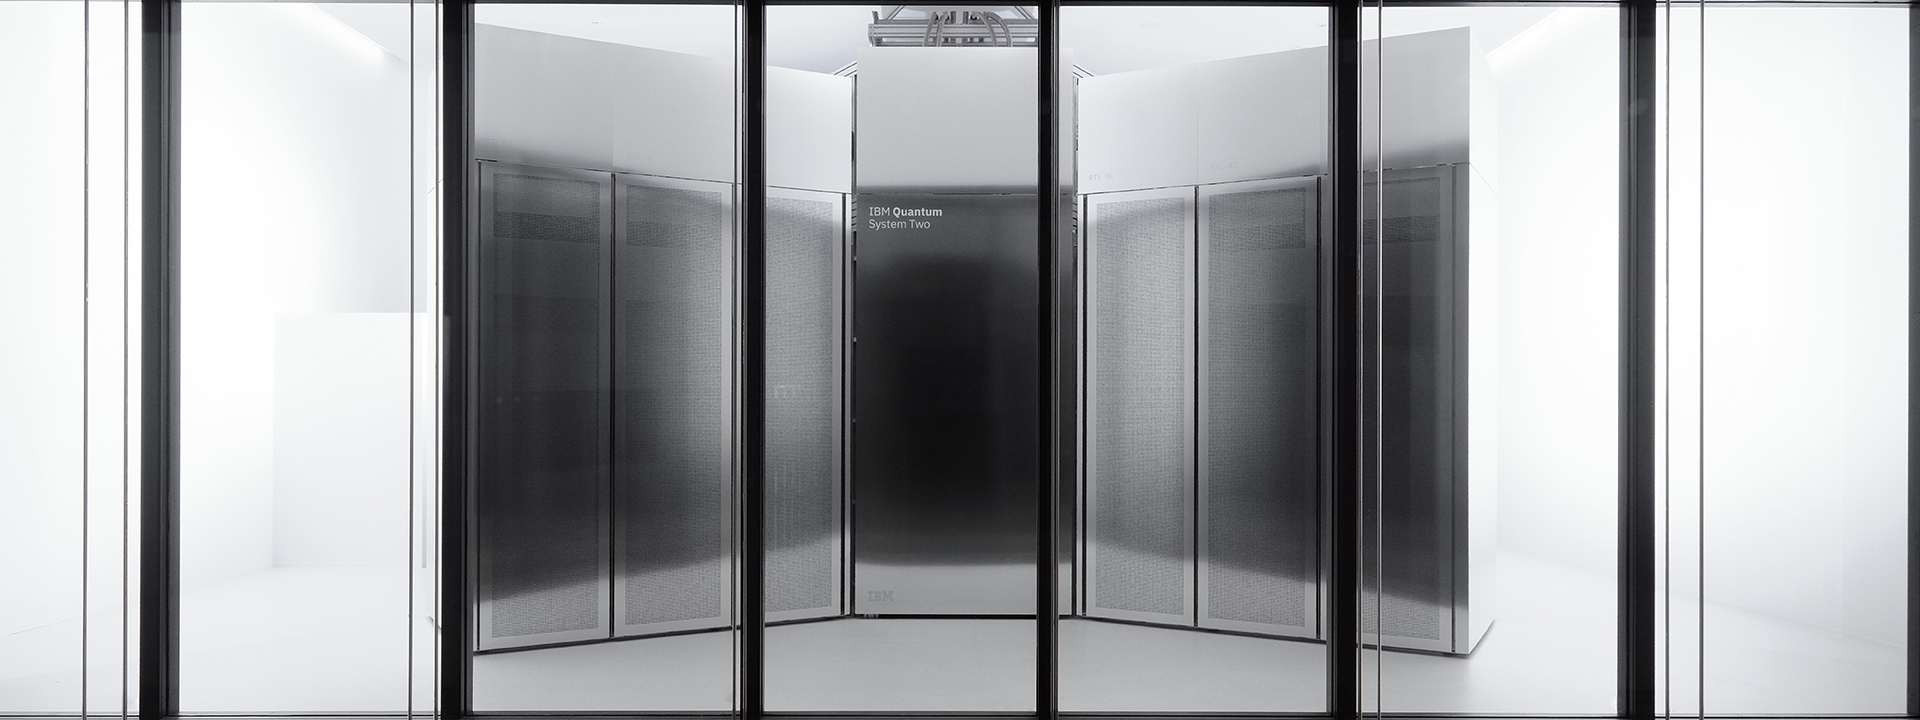
\includegraphics[width=\textwidth]{images/quanten-hardware/IBM-Quantum_System-Two_Riken_banner.jpg}
    \caption{IBM Quantum Computer System Two}
    \label{fig:ibmquantumsystemtwo}
\end{figure}

%Quelle Bild: https://newsroom.ibm.com/2025-06-23-ibm-and-riken-unveil-first-ibm-quantum-system-two-outside-of-the-u-s

\subsubsection{Designphilosophie und Architekturziele}
Im Unterschied zum eher monolithischen Aufbau des IBM Q System One, das primär für den Betrieb eines einzelnen Quantenprozessors (QPU) konzipiert war, wurde das IBM Quantum System Two von Grund auf mit Blick auf mehrere Kernziele entwickelt. 

Zu diesen Zielen zählt erstens die Modularität: Das System ist so strukturiert, dass es aus multiplen, potenziell miteinander verbundenen Modulen aufgebaut werden kann. Dieser Ansatz ermöglicht eine flexible Systemkonfiguration und eine schrittweise Erweiterung der Gesamtanlage. 
Zweitens steht die Skalierbarkeit im Fokus, mit dem Ziel, ein Wachstum auf Tausende von Qubits und darüber hinaus zu ermöglichen. Dies soll durch die Kooperation mehrerer QPUs innerhalb eines oder mehrerer vernetzter Systeme realisiert werden. 
Drittens ist die Konnektivität von essenzieller Bedeutung für die Skalierbarkeit. Darunter wird die Fähigkeit verstanden, QPUs sowohl innerhalb eines Systems als auch systemübergreifend zu verbinden, um die Bearbeitung umfangreicherer und komplexerer Problemstellungen zu ermöglichen.

\begin{figure}[H]
    \centering
    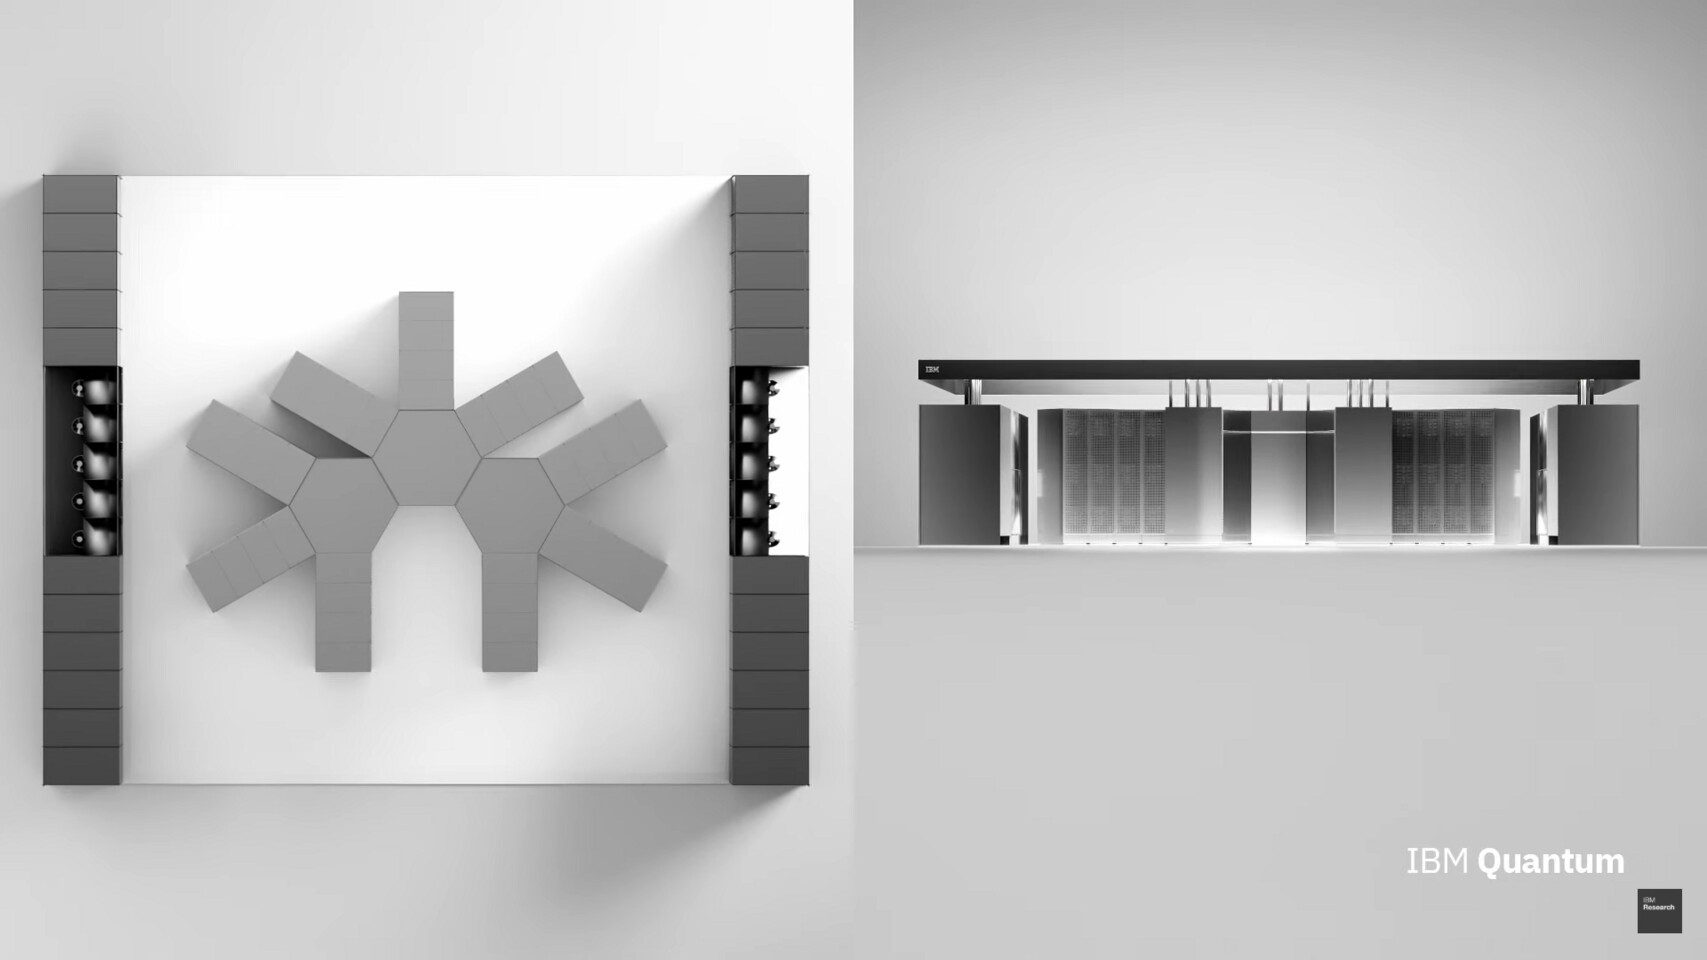
\includegraphics[width=\textwidth]{images/quanten-hardware/IBM_Quantum_System_two_modular.jpg}
    \caption{IBM Quantum Computer System Two: Skalierung und Modularität}
    \label{fig:ibmquantumsystemtwomodular}
\end{figure}

Viertens wurden Aspekte der Servicefreundlichkeit und Aufrüstbarkeit berücksichtigt; das modulare Design ist darauf ausgelegt, Wartungsarbeiten sowie die Implementierung von Hardware-Upgrades zu vereinfachen. Mit dem fünften Kernziel der Hybridität, also der nahtlosen Integration mit klassischer Hochleistungsrechner-Infrastruktur, wird ein zentraler Bestandteil der Vision des Quantum-centric Supercomputing umgesetzt.

\subsubsection{Systemarchitektur und Gehäuse}
Das IBM Quantum System Two weist eine deutlich veränderte äußere Erscheinungsform auf. Die für das System One charakteristische Glaskuppel wurde durch eine umfangreichere, hexagonale Struktur ersetzt. Diese besteht aus hexagonal geformten Basiseinheiten, welche jeweils einen Kryostaten mit Quantenprozessoren sowie die zugehörige unterstützende Infrastruktur aufnehmen können. Die Wahl der hexagonalen Form ist nicht rein ästhetisch motiviert, sondern dient auch funktionalen Zwecken, indem sie die Verbindung mehrerer solcher Einheiten zu größeren Clustern erlaubt (Red Dot Design Award, 2024). 

Jede dieser Einheiten weist Abmessungen von etwa 4,6 Metern in der Höhe und 6,7 Metern in der Breite auf. Die modulare Erweiterung wird dadurch realisiert, dass an die Seitenflächen dieser hexagonalen Einheiten weitere Module angedockt werden können. Diese zusätzlichen Module können entweder weitere QPUs oder klassische Steuer- und Peripherieelektronik enthalten, was ein physisches Wachstum des Systems parallel zur Steigerung der Rechenleistung ermöglicht. Bei den Materialien und dem Design des Gehäuses kommen eloxiertes, poliertes Aluminium sowie Glaselemente zum Einsatz. Die sichtbaren Fugen zwischen den Modulen akzentuieren den modularen Charakter des Systems (iF Design Award, 2024). Das Gesamtdesign zielt darauf ab, Prinzipien der Offenheit und Zugänglichkeit zu vermitteln, während gleichzeitig der Schutz der sensitiven Technologie gewährleistet wird.
%TO-DO: Quellen

\subsubsection{Kryogene Infrastruktur und QPU-Umgebung}
Die Notwendigkeit, eine steigende Anzahl von Qubits bei extrem tiefen Temperaturen – typischerweise im Bereich von 10 bis 20 Millikelvin für supraleitende Qubits – zu betreiben, stellt hohe Anforderungen an die kryogene Infrastruktur. Im Hinblick auf eine skalierbare Kühlung müssen, obgleich die fundamentalen Prinzipien der Dilutionsrefrigeration beibehalten werden, die Kühlleistung und die interne Kapazität der Kryostaten für das Quantum System Two signifikant erhöht werden. 
Dies ist erforderlich, um multiple oder größere QPUs sowie die damit assoziierte Verkabelung und Komponenten, wie beispielsweise Verstärker, adäquat zu versorgen. In diesem Kontext hat IBM auch den „Goldeneye“-Kryostaten erwähnt, einen Dilutionsrefrigerator mit einer besonders großen Kühlkapazität, welcher für die Kühlung zukünftiger Generationen von Multi-Chip-Prozessoren ausgelegt ist (SpinQ, 2025). %To-DO:Quelle richtig hinzufügen
Die Integration von Prozessoren ist ein weiteres Kernelement. Quantum System Two ist dafür konzipiert, mehrere Quantenprozessoren, beispielsweise drei IBM Heron-Prozessoren, in einem einzelnen Kryostaten zu beherbergen und zu betreiben (arXiv, 2024). 
%To-Do: Quellen richtig
\begin{figure}[H]
    \centering
    \includegraphics[width=\textwidth]{images/quanten-hardware/IBM_Quantum_133_Qubit_HERON_03.jpg}
    \caption{IBM 133 Qubit Prozessor Heron}
    \label{fig:ibmheron}
\end{figure}
%Quelle: https://newsroom.ibm.com/2023-12-04-IBM-Debuts-Next-Generation-Quantum-Processor-IBM-Quantum-System-Two,-Extends-Roadmap-to-Advance-Era-of-Quantum-Utility
Eine solche Integration erfordert eine präzise Planung der internen Verkabelung, der thermischen Anbindung und der elektromagnetischen Abschirmung. Das Vibrationsmanagement und die Stabilität gewinnen in einem modularen und potenziell sehr ausgedehnten System zusätzlich an Komplexität und Kritikalität im Vergleich zum System One, um die Kohärenz der Quantenzustände sicherzustellen.

\includepdf[pages=1, fitpaper=true]{GrafikKühlungDeutsch.pdf}


\subsubsection{Signalübertragung, Steuerungselektronik und Konnektivität}
Mit der Zunahme der Anzahl von Qubits und Prozessoren steigen die Anforderungen an die Steuerungs- und Ausleseelektronik sowie an die Verbindungen zwischen den Systemkomponenten exponentiell. %To-do: QUelle
IBM hat eine Steuerungselektronik der dritten Generation entwickelt, die sich durch eine höhere Kompaktheit, gesteigerte Leistungsfähigkeit und eine engere Integration mit den QPUs auszeichnet. Diese Elektronik ist darauf ausgelegt, eine größere Anzahl von Qubits effizient zu steuern und auszulesen (IBM News Room, 2023). %To-Do: quelle hinzufügen
Die Erhöhung der Qubit-Dichte und -Anzahl macht zudem innovative Lösungen für eine hochdichte kryogene Verkabelung notwendig, um die Wärmelast gering zu halten und gleichzeitig eine hohe Signalintegrität zu gewährleisten. Flexible kryogene Hochfrequenzleitungen (CryoFlex) spielen hierbei eine wichtige Rolle. Für die Koordination und das sogenannte „Circuit Knitting“ – ein Verfahren, das große Quantenschaltkreise auf mehrere QPUs aufteilt und klassische Kommunikation von Zwischenergebnissen erfordert, sind leistungsfähige klassische Kommunikationslinks zwischen den Prozessoren und den Steuerungseinheiten unerlässlich. %To-Do: Quelle
Langfristig verfolgt IBM das Ziel, auch direkte quantenkohärente Verbindungen (Quantum Links) zwischen QPUs zu realisieren, um echte verteilte Quantenberechnungen über mehrere Chips hinweg zu ermöglichen (IBM Quantum Roadmap).

\subsubsection{Integration klassischer und quantenmechanischer Komponenten}
Das IBM Quantum System Two ist als zentrales Element einer „Quantum-centric Supercomputing“-Architektur konzipiert. Dies impliziert, dass das System für eine enge Kooperation mit klassischen Supercomputern und Cloud-Ressourcen ausgelegt ist, um hybride Workflows zu unterstützen. Middleware und Software-Werkzeuge wie Qiskit werden kontinuierlich weiterentwickelt, um solche hybriden Quanten-Klassik-Workflows effizient zu orchestrieren, Rechenaufgaben dynamisch zu verteilen und Ergebnisse zu konsolidieren (The Quantum Insider, 2024). %To-Do: QUelle
Der Ansatz des Quantum Serverless zielt darauf ab, Quanten- und klassische Berechnungen nahtlos in unterschiedlichen Umgebungen, sei es in der Cloud oder on-premises, zu integrieren und auszuführen.

\subsubsection{Wartung, Skalierbarkeit und Modularität in der Praxis}
Die praktische Umsetzung der Prinzipien von Modularität und Skalierbarkeit stellt einen Hauptfokus bei der Entwicklung des IBM Quantum System Two dar. Das System ist für eine phasenweise Inbetriebnahme (Phased Deployment) und für Upgrades konzipiert. Dies bedeutet, dass es schrittweise ausgebaut und mit neueren Prozessorgenerationen (wie den in der IBM Roadmap genannten zukünftigen Prozessoren Flamingo oder Kookaburra) oder verbesserter Steuerungshardware aufgerüstet werden kann, ohne dass ein Austausch des Gesamtsystems notwendig wird. Das Design berücksichtigt ferner die Notwendigkeit regelmäßiger Wartung durch entsprechend gestaltete Servicezugänge, die den Zugriff auf kritische Komponenten erleichtern. Über spezifische Wartungsprozeduren sind, ähnlich wie beim System One, öffentlich meist nur allgemeine Informationen verfügbar.

\subsubsection{Relevante Designentscheidungen aus Ingenieursperspektive}
Mehrere zentrale Designentscheidungen prägen die ingenieurtechnische Ausrichtung des IBM Quantum System Two. Die Priorisierung der Modularität stellt hierbei die fundamentalste und weitreichendste Entscheidung dar, welche die Skalierbarkeit und Zukunftsfähigkeit des Systems gewährleisten soll. Parallel dazu wurde ein starker Fokus auf die Interkonnektivität gelegt; die Fähigkeit, Prozessoren und Systeme miteinander zu verbinden, ist entscheidend, um die Limitierungen einzelner QPUs zu überwinden. Die Entwicklung des Systems folgt einem integrierten Ansatz, bei dem Hardware, Software (einschließlich Qiskit und Middleware), Steuerung und klassische Computerressourcen als eine kohärente Einheit betrachtet und entwickelt werden. Schließlich schafft die Architektur des Quantum System Two, obwohl sie selbst noch nicht die Ära der vollständigen Fehlertoleranz einläutet, die notwendige Skalierbarkeit und Komplexität, um fortgeschrittene Fehlerminderungs- und Quantenfehlerkorrekturcodes zu implementieren und zu testen. %To-do: Quelle
\\\\
Das IBM Quantum System Two stellt somit einen entscheidenden Evolutionsschritt dar. Es legt die technologischen Grundlagen für Quantencomputer, die potenziell in der Lage sein werden, Probleme von praktischer Relevanz zu lösen, welche für klassische Supercomputer als unlösbar gelten. Die Realisierung dieser Vision ist maßgeblich von der erfolgreichen Bewältigung der komplexen ingenieurtechnischen Herausforderungen in den Bereichen Skalierung, Konnektivität und Systemintegration abhängig.


\printbibliography


